% ============================================================
%  Journal of Electrical Engineering & Technology (JEET) Format
%  Vehicle-to-Vehicle Communication for Blind Spot Detection
% ============================================================
\documentclass[sn-mathphys-num,Numbered,iicol]{sn-jnl}

% ---- Core Packages ----
\usepackage[T1]{fontenc}
\usepackage[utf8]{inputenc}
\usepackage{amsmath,amssymb,amsfonts}
\usepackage{algorithmic}
\usepackage{graphicx}
\usepackage{textcomp}
\usepackage{booktabs}
\usepackage{array}
\usepackage{url}
\usepackage{mathptmx}  % Times New Roman font (as per JEET template)

% ---- Custom math operator ----
\DeclareMathOperator{\atan2}{atan2}

% ============================================================
\begin{document}

\title[V2V Blind Spot Detection via Severity-Gated CRI]{Vehicle-to-Vehicle Communication for Blind Spot Detection and
Accident Prevention Using Severity-Gated Collision Risk Indexing}

\author*[1]{\fnm{Omkar} \sur{Kadam}}\email{omkarkadam181188@gmail.com}
\author[1]{\fnm{Abhinav} \sur{Prasad}}
\author[1]{\fnm{Gauri} \sur{Phanse}}
\author[1]{\fnm{Afraz} \sur{Khan}}
\author[1]{\fnm{Vaishali} \sur{Khairnar}}\email{vaishali.khairnar@ternaengg.ac.in}

\affil[1]{\orgdiv{Department of Information Technology},
\orgname{Terna Engineering College},
\orgaddress{\city{Nerul, Navi Mumbai}, \country{India}}}

% ============================================================
% ABSTRACT
% ============================================================
\abstract{Blind spot accidents during lane changes are a major cause of urban traffic collisions. Current driver-assistance systems using radar or cameras fail when other vehicles block the line of sight. This paper presents a Vehicle-to-Vehicle (V2V) Blind Spot Detection system using wireless communication to detect nearby vehicles even when hidden from sensors. The system uses only 5 data fields from the standard Basic Safety Message (BSM) --- far fewer than the 13 fields required by previous systems. We introduce a Collision Risk Index (CRI) with a severity gate that prevents false alarms by requiring at least one danger signal to be genuinely high before triggering a warning. Tested using 146,051 simulated vehicle interactions on a real road network, it achieved an AUC of 0.9869 (AUPRC = 0.677 vs.\ 0.024 random baseline), confirmed stable across six independent traffic seeds ($0.9954 \pm 0.0041$). An exploratory XGBoost classifier is included as a future-work baseline.}

\keywords{Blind Spot Detection, Collision Risk Index, DSRC/C-V2X, Severity Gate, Vehicle-to-Vehicle Communication}

\maketitle

% ============================================================
% 1. INTRODUCTION
% ============================================================
\section{Introduction}\label{sec:introduction}

Road traffic injuries cause about 1.19 million deaths worldwide every year, making it the leading cause of death for people aged 5--29~\cite{who2023}. Many of these accidents happen when drivers change lanes without seeing vehicles in their blind spots. In India, dense and mixed traffic on urban roads makes this problem even worse~\cite{morth2023}.

While modern driver-assistance systems use radar and cameras to detect blind spot vehicles, these sensors fail when large vehicles physically block the view --- which happens frequently in heavy traffic~\cite{biswas2006}. Vehicle-to-Vehicle (V2V) communication solves this by letting vehicles exchange data using radio signals that pass through obstacles. Each vehicle broadcasts its location, speed, and other data using the Basic Safety Message (BSM)~\cite{sae_j2735,sae_j2945} at 10~Hz, reaching up to 300~m~\cite{biswas2006}. Two wireless technologies support this: DSRC using IEEE 802.11p~\cite{ieee_80211p}, and C-V2X using cellular networks~\cite{3gpp2016}.

Previous V2V blind spot systems needed up to 13 BSM fields including heading, turn signals, and yaw rate~\cite{mousa2021}, creating compatibility problems with older vehicles. Our system uses only 5 fields: GPS position ($x$, $y$), speed ($v$), acceleration ($a$), and braking ($d$), deriving heading from position history.

The main contributions are:
\begin{enumerate}
  \item \textbf{Severity-gated Collision Risk Index.} A risk formula requiring at least one genuinely high danger signal before triggering a warning, preventing false alarms from small values adding up.
  \item \textbf{Minimal 5-field BSM.} Eliminates the need for 13 fields, making the system compatible with all vehicle types.
  \item \textbf{Exploratory ML baseline comparison.} An XGBoost classifier reveals that physics models outperform data-driven approaches when dangerous events are rare.
  \item \textbf{Realistic testing.} Tested on a real road network with traffic signal violations, narrow hilly roads, and simulated communication failures.
\end{enumerate}

% ============================================================
% 2. RELATED WORK
% ============================================================
\section{Related Work}\label{sec:related}

\subsection{Sensor-Based and V2V Blind Spot Detection}
Current commercial systems use radar sensors on rear bumpers, which work well on open roads but fail in dense traffic where large vehicles block signals. V2V communication overcomes this as radio signals pass through vehicles. V2V systems use SAE J2735~\cite{sae_j2735} for message formatting and IEEE 802.11p~\cite{ieee_80211p} for transmission. The SAE J2945/1 standard~\cite{sae_j2945} requires 10~Hz BSM broadcasts. Our system uses only 5 BSM Part~I fields, compatible with basic on-board units~\cite{festag2014}.

\subsection{Risk Assessment and Machine Learning}
Time-to-Collision (TTC) is widely used in Euro NCAP testing~\cite{euroncap2019} but becomes unreliable with lateral vehicle movement. Early V2V systems used shared GPS coordinates~\cite{rawashdeh2008}; Kim~\textit{et~al.}~\cite{kim2015} developed threat assessment using V2V data; Mousa~\textit{et~al.}~\cite{mousa2021} created a 13-field V2V blind spot system. A common problem is that multiple small risk values trigger false warnings --- our severity gate prevents this. Machine learning models like XGBoost~\cite{chen2016xgboost} work well for structured data, but raise interpretability concerns for safety decisions. SMOTE~\cite{smote2002} helps handle rare dangerous events. In our system, an XGBoost classifier is included as an exploratory comparison only.

% ============================================================
% 3. SYSTEM ARCHITECTURE
% ============================================================
\section{System Architecture}\label{sec:architecture}

The system is organized as a four-layer pipeline (Fig.~\ref{fig:architecture}):
\textbf{Layer~1 (Simulation):} Eclipse SUMO~\cite{sumo2018} generates vehicle movements at 10~Hz with injected danger scenarios.
\textbf{Layer~2 (Communication):} Vehicle data is packaged into 5-field BSMs with GPS noise (1.5~m) and packet drops (Gilbert-Elliott model). Lost messages trigger dead-reckoning prediction.
\textbf{Layer~3 (Intelligence):} Two parallel paths process received data --- a physics model (primary, CRI-based) and an XGBoost classifier (exploratory baseline).
\textbf{Layer~4 (Analytics):} A Streamlit dashboard displays real-time V2V connections and risk scores.

\begin{figure}[htbp]
  \centering
  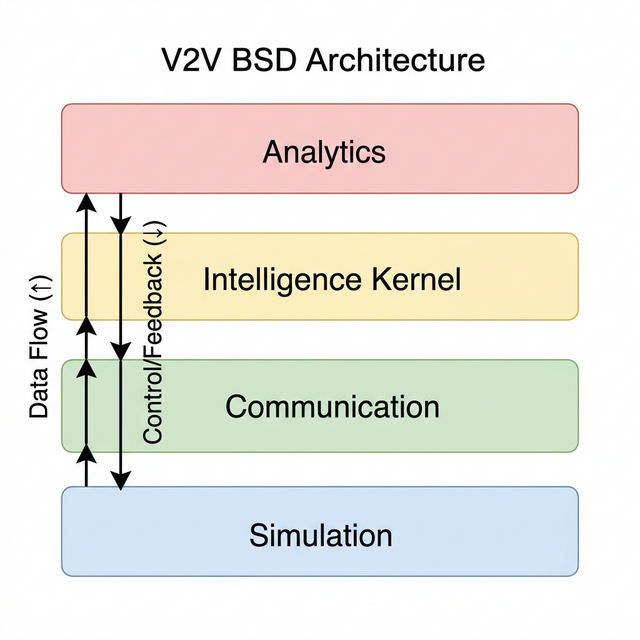
\includegraphics[width=0.9\columnwidth]{architecture_diagram.png}
  \caption{Four-layer V2V BSD system architecture.}
  \label{fig:architecture}
\end{figure}

% ============================================================
% 4. MATHEMATICAL MODEL
% ============================================================
\section{Mathematical Model}\label{sec:math}

The system takes 5 data fields from each nearby vehicle and produces a risk score between 0 (safe) and 1 (critical).

\subsection{BSM Input and Heading Estimation}
The 5-field BSM is $\mathrm{BSM} = \{x, y, v, a, d\}$ where $x,y$ are GPS coordinates, $v$ is speed, $a$ is acceleration, and $d$ is braking strength. Heading is derived from position history:
\begin{equation}
  \theta(t) = \atan2\!\bigl(y(t)-y(t-1),\; x(t)-x(t-1)\bigr)
\end{equation}
At speeds below 0.5~m/s, the last known heading is held to avoid GPS noise. The turning rate is $\dot{\theta}(t) = [\theta(t) - \theta(t-1)]/\Delta t$.

\subsection{Coordinate Transformation and Blind Spot Zone}
The target's position is transformed into the ego vehicle's reference frame:
\begin{align}
  x_{\mathrm{rel}} &= \sin(\theta_e)\cdot\Delta x - \cos(\theta_e)\cdot\Delta y \\
  y_{\mathrm{rel}} &= \cos(\theta_e)\cdot\Delta x + \sin(\theta_e)\cdot\Delta y
\end{align}
where $\Delta x = x_t - x_e$, $\Delta y = y_t - y_e$. The blind spot zone extends with speed:
\begin{equation}
  L_{\mathrm{bs}}(v_e) = L_{\mathrm{base}} + \lambda_{\mathrm{scale}}
    \cdot \mathrm{clamp}\!\left(\frac{v_e - v_{\min}}{v_{\max} - v_{\min}},\,0,\,1\right)
\end{equation}
where $L_{\mathrm{base}} = 4.5$~m is the minimum zone length and $\lambda_{\mathrm{scale}} = 12.0$~m is the speed-dependent extension. On curves, a curvature correction shifts the zone laterally: $x_{\mathrm{corrected}} = x_{\mathrm{rel}} - y_{\mathrm{rel}}^2\dot{\theta}_e/(2v_e)$.

\subsection{Blind Spot Zone Probability}
Since GPS has 1.5~m uncertainty, the system calculates the \textit{probability} of a target being in the blind spot using Gaussian integration:
\begin{align}
  P_{\mathrm{lat}} &= \Phi\!\left(\frac{x_{\max} - x_c}{\sigma}\right) - \Phi\!\left(\frac{x_{\min} - x_c}{\sigma}\right) \\
  P_{\mathrm{lon}} &= \Phi\!\left(\frac{y_{\max} - y_c}{\sigma}\right) - \Phi\!\left(\frac{y_{\min} - y_c}{\sigma}\right)
\end{align}
where $\Phi$ is the standard normal CDF and $\sigma = 1.5$~m. The combined probability is $P_{\mathrm{gps}} = |P_{\mathrm{lat}}| \times P_{\mathrm{lon}}$, with a forward-lane filter to prevent false alarms from vehicles directly ahead.

\subsection{Dead Reckoning and Packet Loss}
When packets are lost, the system predicts target position using a Constant-Acceleration, Constant-Yaw-Rate model:
\begin{equation}
  \hat{x} = x + v\cos(\theta)\,\tau + \tfrac{1}{2}\,a_{\mathrm{net}}\cos(\theta)\,\tau^2
\end{equation}
\begin{equation}
  \hat{y} = y + v\sin(\theta)\,\tau + \tfrac{1}{2}\,a_{\mathrm{net}}\sin(\theta)\,\tau^2
\end{equation}
Prediction is limited to 0.5~s; targets are dropped after four consecutive lost packets. A Packet Loss Ratio (PLR) tracked over a 10-step window increases risk: $\Gamma_{\mathrm{plr}} = 1 + 0.30 \cdot \mathrm{PLR}_{\mathrm{window}}$.

\subsection{Deceleration Risk ($R_{\mathrm{decel}}$)}
This component measures whether the target vehicle can stop in time. The maximum braking capability is calculated considering both road friction and aerodynamic drag:
\begin{equation}
  a_{\max} = \mu\cdot g + \frac{\rho\cdot C_d\cdot A_f\cdot v_t^2}{2\cdot M_t}
\end{equation}
where $\mu$ is road friction, $g$ is gravity, and the second term accounts for air resistance. The total stopping distance includes a 1.2~second reaction time~\cite{aashto2018}:
\begin{equation}
  D_{\mathrm{stop}} = v_t\cdot T_{\mathrm{react}} + \frac{v_t^2}{2\cdot a_{\max}}
\end{equation}
The risk grows exponentially as the stopping distance approaches the actual gap between vehicles:
\begin{equation}
  R_{\mathrm{decel}} = \mathrm{clip}\!\left(
    \exp\!\left(-K_{\mathrm{brake}} \cdot \frac{d_{\mathrm{gap}} - D_{\mathrm{stop}}}{D_{\mathrm{stop}}}\right),\; 0,\; 1
  \right)
\end{equation}
where $K_{\mathrm{brake}} = 1.50$. When the gap exactly equals the stopping distance, risk is 1.0; as the gap grows, risk drops toward zero.

\subsection{Time-to-Collision Risk ($R_{\mathrm{ttc}}$)}
This measures how soon a collision could happen. The system solves the equation $a_{\mathrm{rel}}\,\tau^2 + v_{\mathrm{rel}}\,\tau + x_{\mathrm{rel}} = 0$ to find TTC:
\begin{equation}
  R_{\mathrm{ttc}} = \begin{cases}
    1.0 & \text{if } \mathrm{TTC} \le 4.0\;\text{s} \\[2pt]
    (4.0/\mathrm{TTC})^{2} & \text{if } 4.0 < \mathrm{TTC} \le 8.0\;\text{s} \\[2pt]
    0 & \text{otherwise}
  \end{cases}
\end{equation}
A parallel calculation checks for side collisions using the lateral gap. For the lateral TTC component, a linear decay $1 - \mathrm{TTC}_{\mathrm{lat}}/\mathrm{TTC}_{\mathrm{crit}}$ is used rather than the quadratic form, as lateral closing speeds are typically lower. The combined TTC risk takes the higher of the two values.

\subsection{Intent Risk ($R_{\mathrm{intent}}$)}
Without turn signal data, the system estimates whether the ego vehicle is drifting sideways toward another lane:
\begin{equation}
  R_{\mathrm{intent}} = 0.6 \cdot \min\!\left(1,\; \frac{\max(0,\, v_{\mathrm{lat,toward}})}{1.0\;\text{m/s}}\right)
\end{equation}
However, testing showed that predicting lane-change intent without turn signals is unreliable. Therefore, this component is disabled in the final system ($\gamma=0$).

The distributions of all three risk components across the simulation are shown in Fig.~\ref{fig:risk_components}. High-risk values are rare, consistent with the 2.37\% positive event rate.

\begin{figure}[htbp]
  \centering
  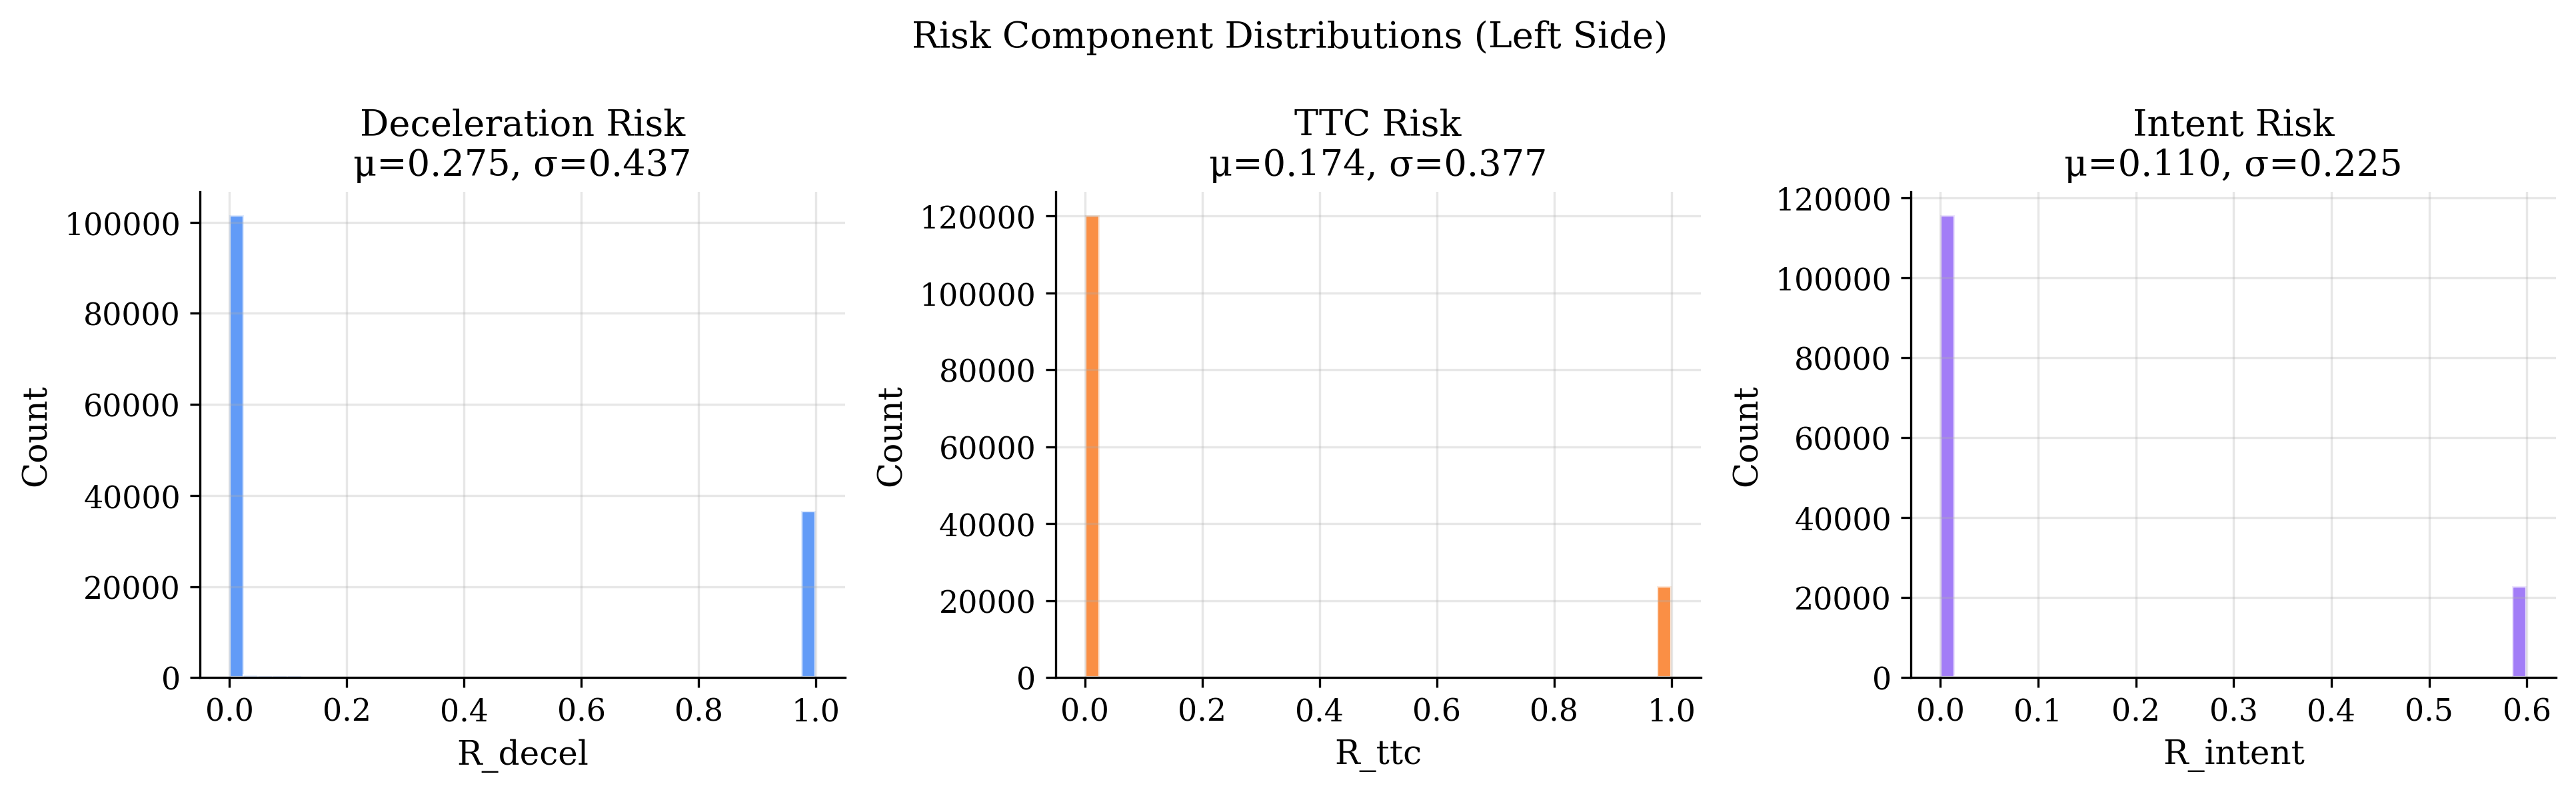
\includegraphics[width=0.9\columnwidth]{fig5_risk_components.png}
  \caption{Distributions of the three CRI risk components. High-risk values are rare, consistent with the 2.37\% positive event rate in the simulation.}
  \label{fig:risk_components}
\end{figure}

\subsection{CRI with Severity Gate}
The final Collision Risk Index combines all components:
\begin{equation}
  \mathrm{CRI} = \mathrm{clip}\!\Big(
    P_{\mathrm{gps}} \cdot \max(R_{\mathrm{decel}},R_{\mathrm{ttc}})
    \cdot \bigl[\alpha R_{\mathrm{decel}} + \beta R_{\mathrm{ttc}}
               + \gamma R_{\mathrm{intent}}\bigr]
    \cdot \Gamma_{\mathrm{plr}},\;0,\;1\Big)
\end{equation}
The $\max(R_{\mathrm{decel}},R_{\mathrm{ttc}})$ \textbf{severity gate} prevents false alarms from small harmless values adding up by requiring at least one genuinely high danger signal. Optimized weights: $\alpha=0.20$, $\beta=0.80$, $\gamma=0.00$.

\subsection{Alert Levels}
The system triggers four alert levels based on CRI:
\begin{itemize}
  \item \textbf{SAFE} (CRI $< 0.30$): No danger detected
  \item \textbf{CAUTION} (CRI $\ge 0.30$): Vehicle detected in blind spot
  \item \textbf{WARNING} (CRI $\ge 0.60$): Close proximity or approach
  \item \textbf{CRITICAL} (CRI $\ge 0.80$): Imminent collision risk
\end{itemize}
To prevent alerts from flickering on and off, the system requires 3 consecutive steps above a threshold before upgrading, and a small buffer band (0.05) before downgrading. Left and right sides are monitored independently. The CRI distribution (Fig.~\ref{fig:cri_dist}) confirms 96.0\% of observations remain SAFE.

\begin{figure}[htbp]
  \centering
  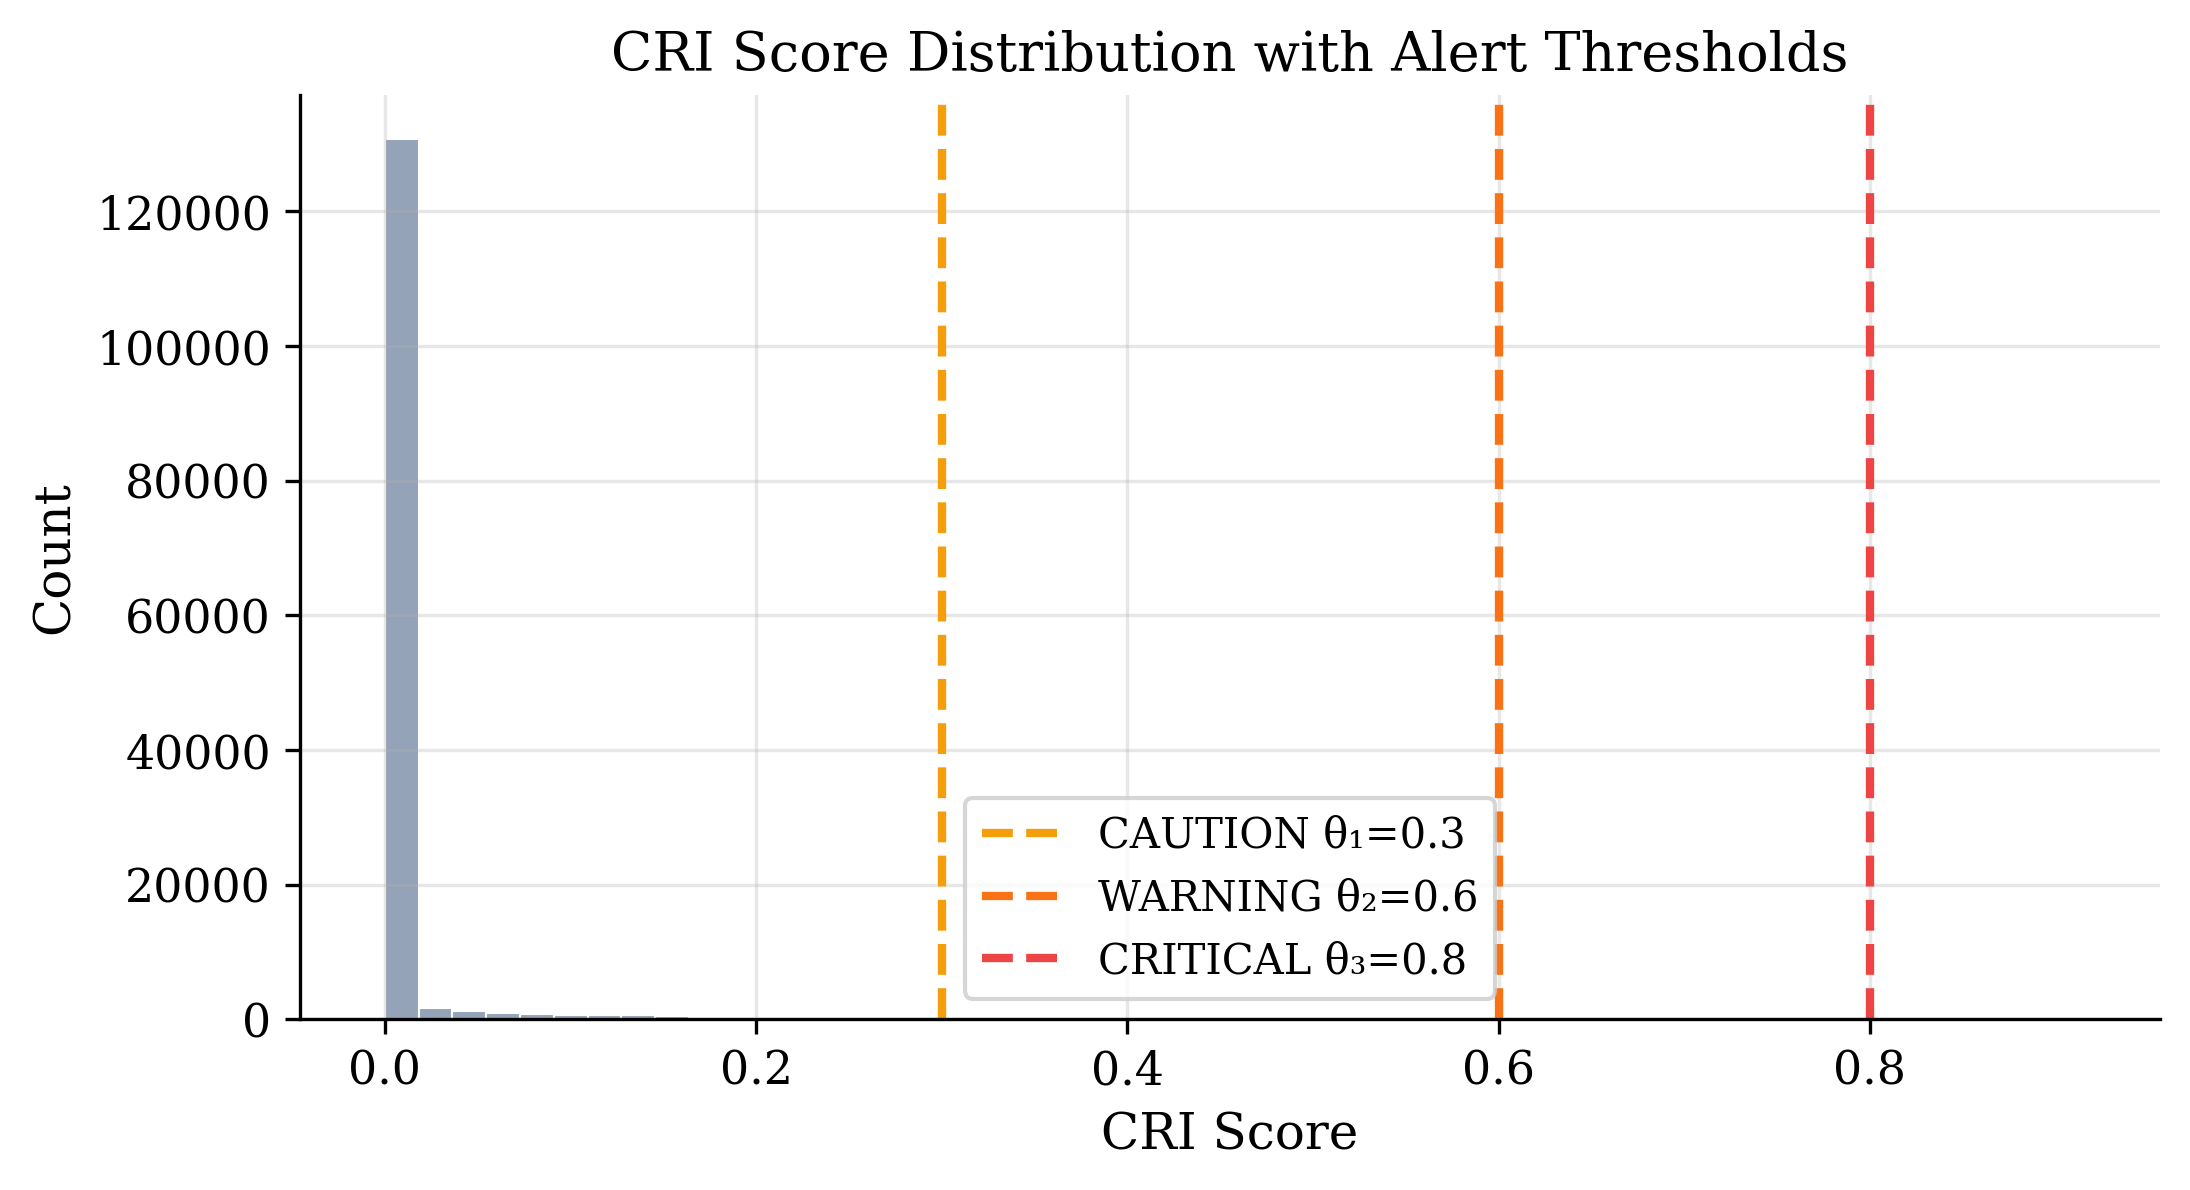
\includegraphics[width=0.9\columnwidth]{fig2_cri_distribution.png}
  \caption{CRI score distribution across 146,051 timesteps. 96.0\% remain in the SAFE region, confirming the severity gate prevents excessive warnings.}
  \label{fig:cri_dist}
\end{figure}

Fig.~\ref{fig:alert_timeline} shows the alert activity over the full simulation, with spikes corresponding to injected danger scenarios. Fig.~\ref{fig:cri_ts} illustrates the CRI time-series for a single vehicle pair, showing how the hysteresis mechanism prevents alert flickering during risk escalation and de-escalation.

\begin{figure}[htbp]
  \centering
  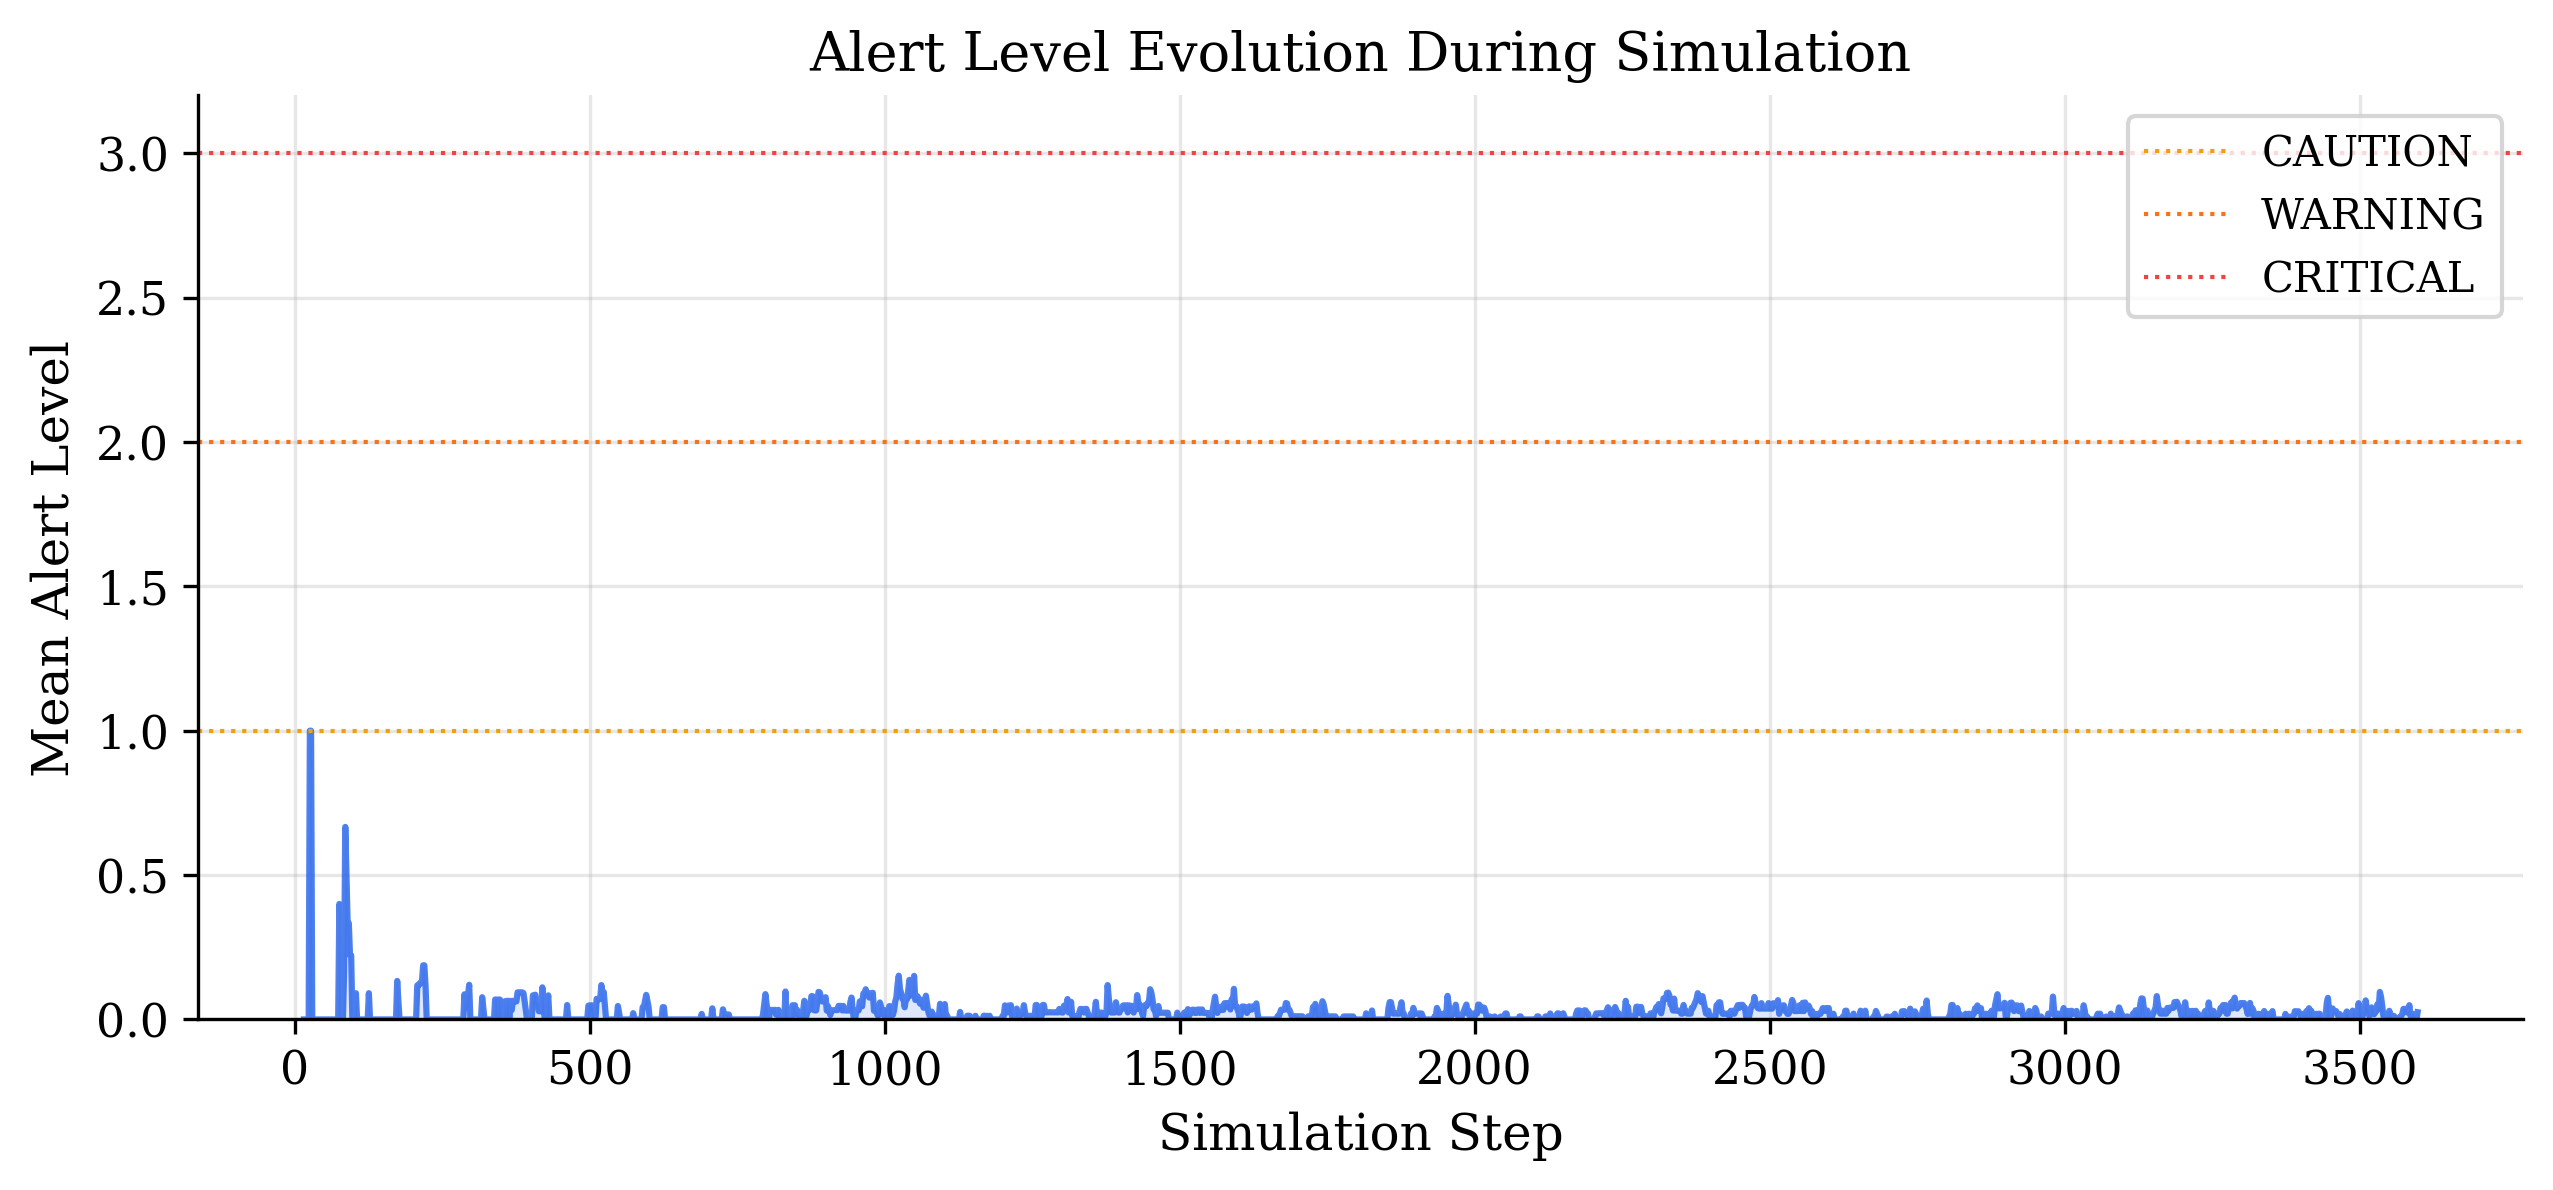
\includegraphics[width=0.9\columnwidth]{fig4_alert_timeline.png}
  \caption{Mean alert level over the 360-second simulation. Spikes correspond to injected danger scenarios (traffic signal violations and narrow road events).}
  \label{fig:alert_timeline}
\end{figure}

\begin{figure}[htbp]
  \centering
  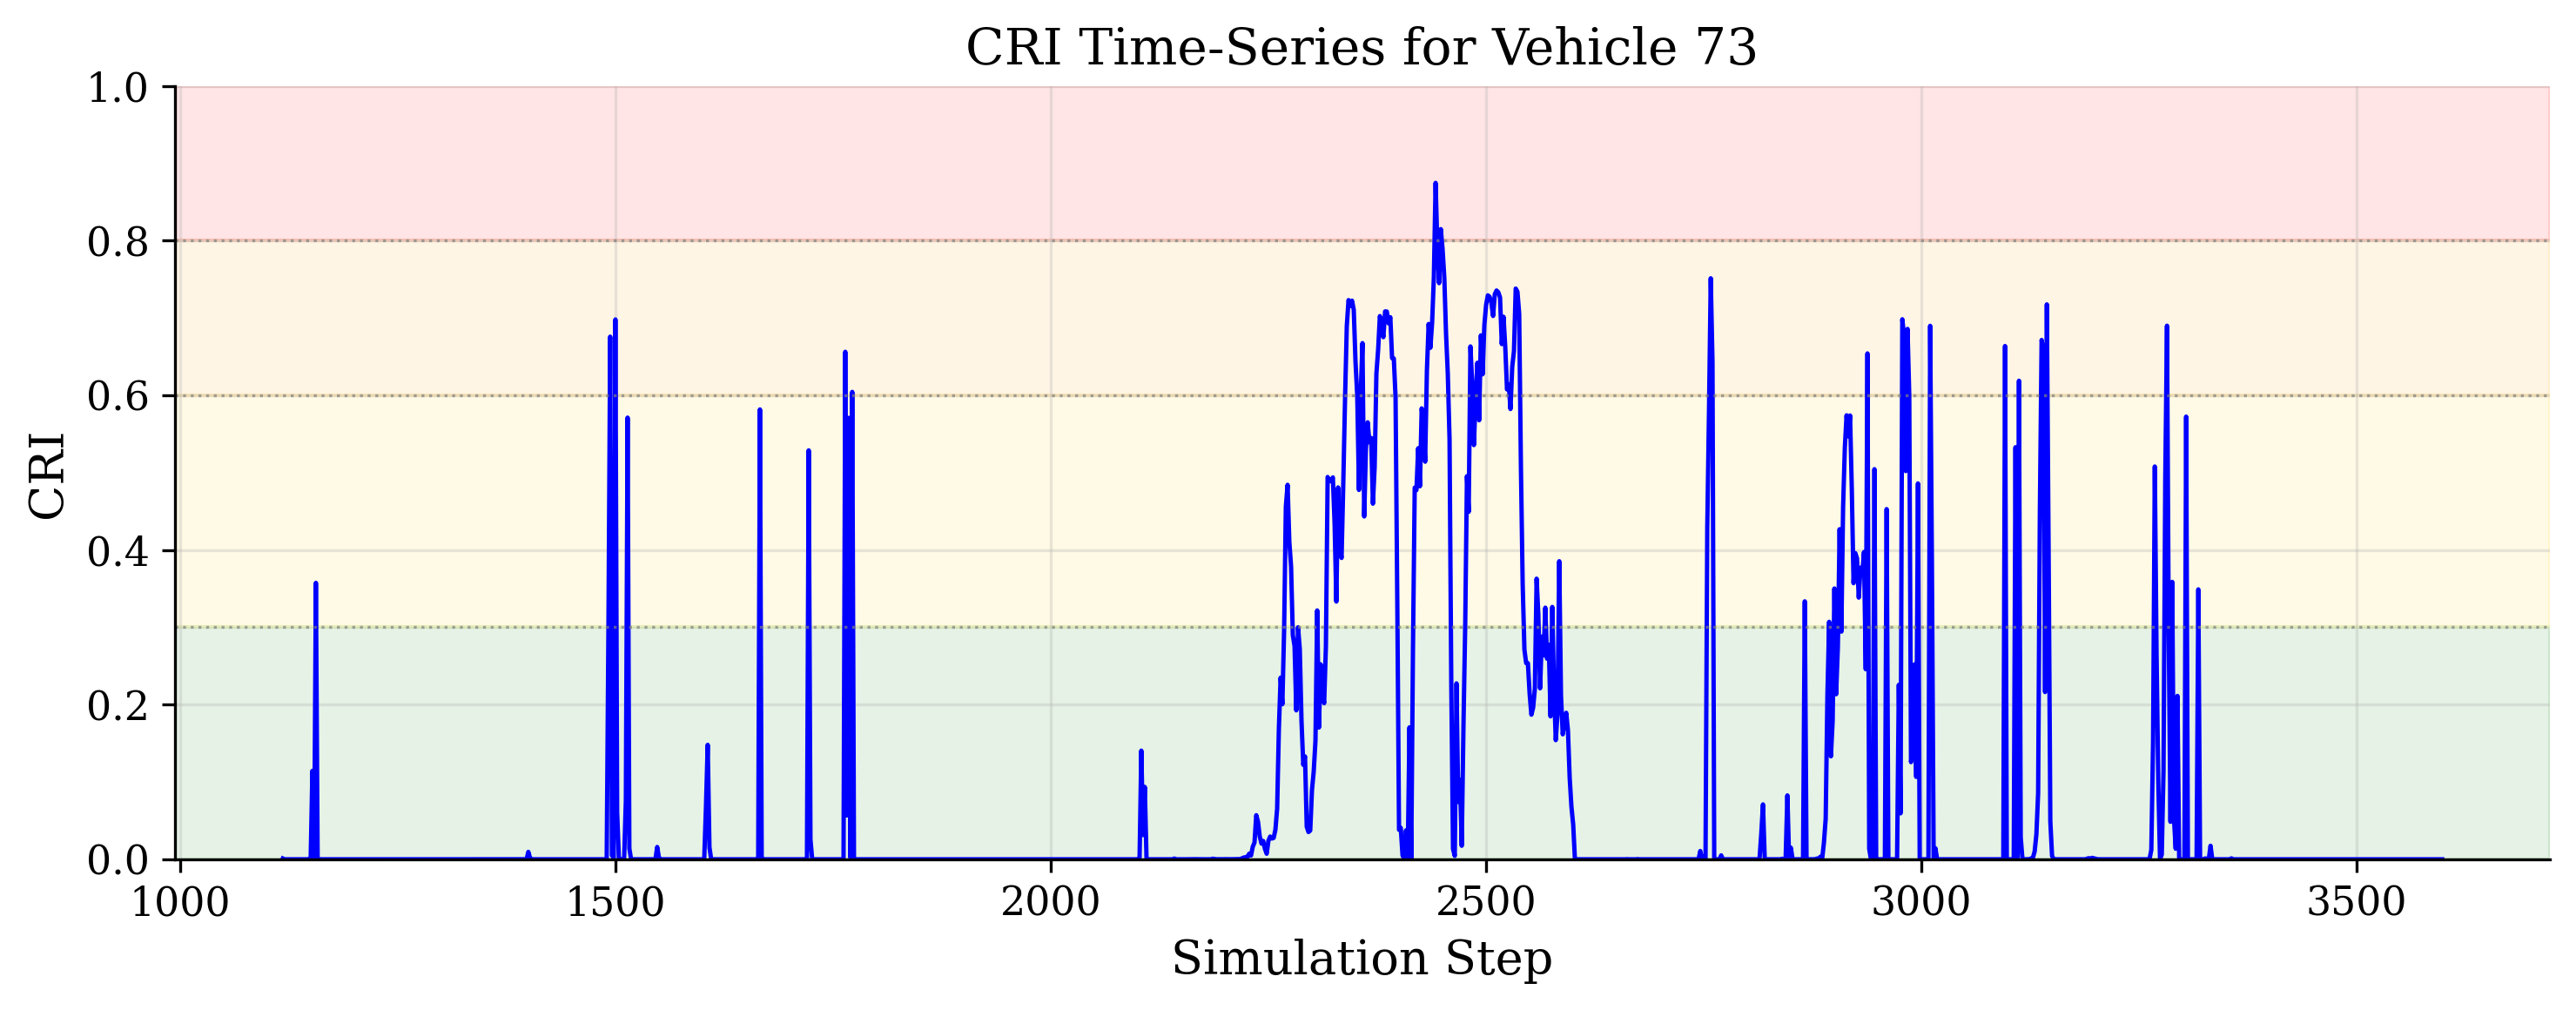
\includegraphics[width=\columnwidth]{fig10_cri_timeseries.png}
  \caption{CRI time-series for a single vehicle showing risk escalation and de-escalation. Horizontal lines indicate alert thresholds: CAUTION (0.30), WARNING (0.60), CRITICAL (0.80). The hysteresis requirement (3 consecutive steps) delays alert upgrades, preventing flicker.}
  \label{fig:cri_ts}
\end{figure}

% ============================================================
% 5. SCENARIO MODELLING
% ============================================================
\section{Scenario Modelling}\label{sec:scenario}

To test the system under realistic danger conditions, two conflict scenarios and a communication failure model were implemented.

\subsection{Traffic Signal Violation (TSV)}
When a vehicle approaches an intersection during a red light, there is a 30\% chance it will ignore the signal and continue at full speed. This creates dangerous crossing conflicts that test the system's ability to detect side-impact collision risks.

\subsection{Hilly Narrow Road (HNR)}
On selected road segments, lane width is reduced to 2.8~metres and road friction is lowered to 0.55 (simulating wet or hilly conditions). Some vehicles (10\% probability) attempt aggressive overtaking. This tests the system's ability to handle reduced braking capability and tight lateral spaces.

\subsection{Communication Packet Loss}
Real-world wireless signals can be interrupted by buildings, other vehicles, or interference. This is modelled using a Gilbert-Elliott two-state channel~\cite{gilbert1960}: in the good state, only 1\% of packets are lost; in the bad state, 50\% are lost. The system spends about 9.1\% of the time in the bad state, creating realistic multi-packet outages that test the dead-reckoning prediction.

The effect of these scenarios on risk levels is shown in Fig.~\ref{fig:scenario_cri}. TSV events cause periodic spikes at intersections; HNR conditions cause sustained elevated risk from reduced friction and narrow lanes.

\begin{figure}[htbp]
  \centering
  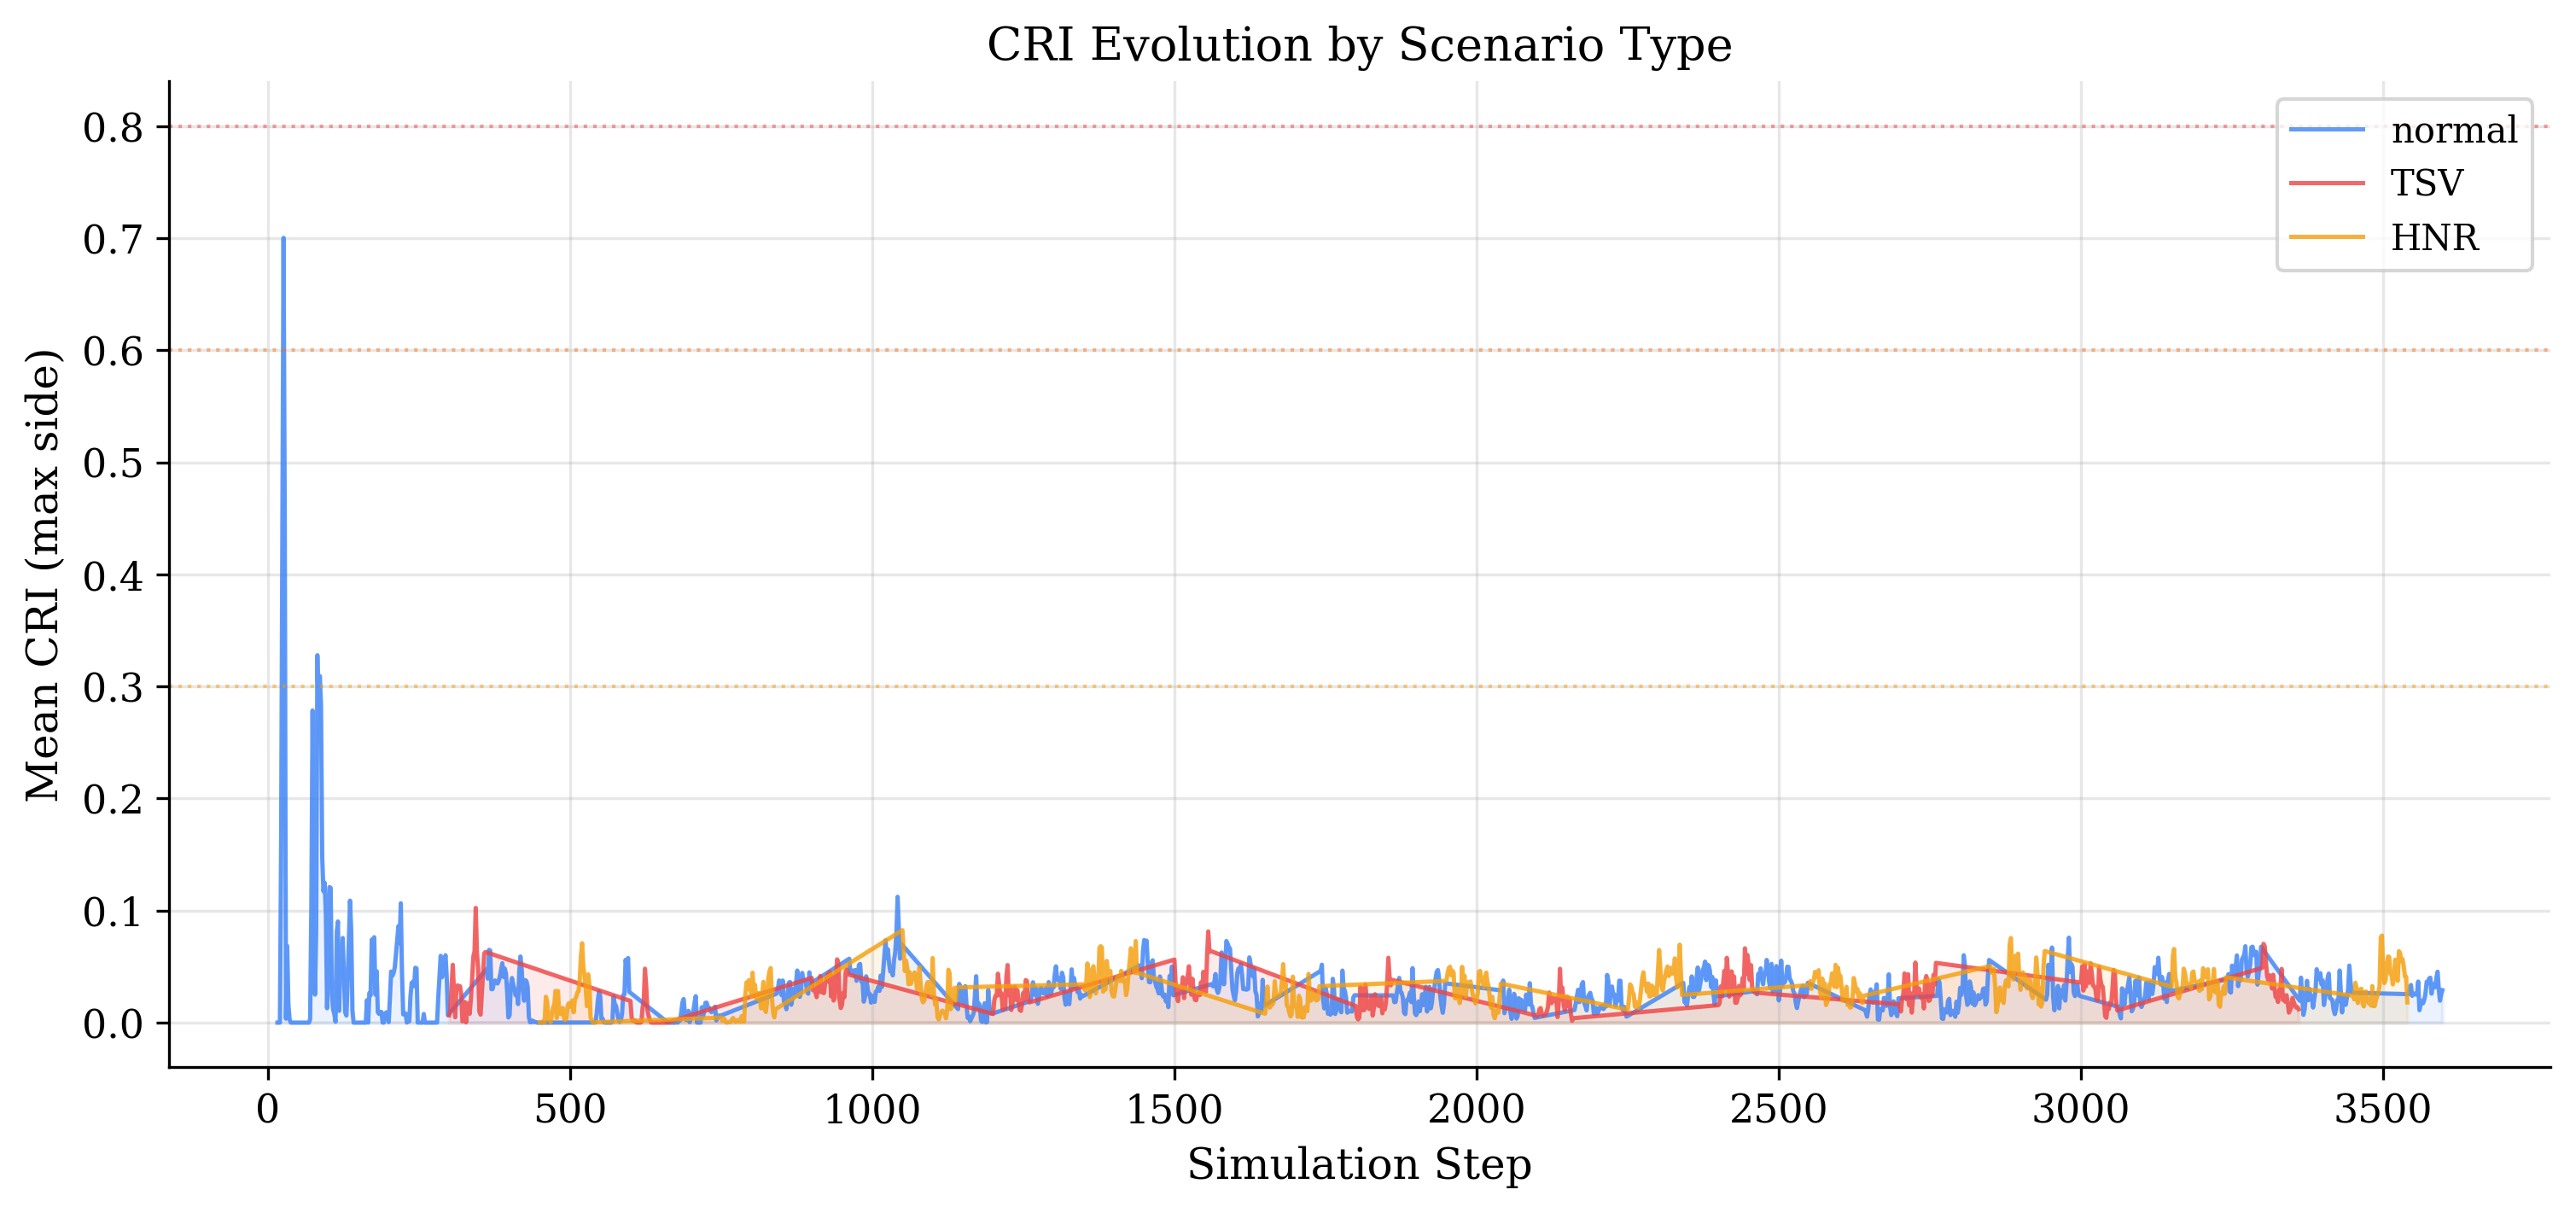
\includegraphics[width=0.9\columnwidth]{fig6_scenario_comparison.png}
  \caption{Mean CRI over time by scenario type. TSV events cause periodic spikes at intersections; HNR conditions cause sustained elevated risk.}
  \label{fig:scenario_cri}
\end{figure}

% ============================================================
% 6. EXPERIMENTAL SETUP
% ============================================================
\section{Experimental Setup}\label{sec:setup}

\subsection{Simulation Environment}
All experiments use Eclipse SUMO~\cite{sumo2018} traffic simulator running at 10~Hz (10 updates per second). The road network is a 539-edge map of the Atal Bridge corridor in Navi Mumbai, India, extracted from OpenStreetMap. The simulation runs for 360 seconds with up to 163 simultaneous vehicles, producing 146,051 total observations. All experiments use random seed 42 for reproducibility.

\subsection{Road Network}
The Atal Bridge network includes multi-lane roads, controlled intersections, and highway ramps --- significantly more complex than the simple highway segments commonly used in V2V research. The simulated traffic models Indian conditions: high vehicle density, mixed vehicle types (sedans, SUVs, trucks), and frequent lane changes.

\subsection{Parameter Reference Table}
All system parameters are listed in Table~\ref{tab:params}.

\begin{table}[htbp]
  \caption{System Parameter Reference}
  \label{tab:params}
  \renewcommand{\arraystretch}{1.15}
  \begin{tabular}{@{}lccl@{}}
    \toprule
    \textbf{Parameter} & \textbf{Symbol} & \textbf{Value} & \textbf{Unit} \\
    \midrule
    BSM Frequency       & $1/\Delta t$              & 10   & Hz  \\
    Detection Range     & $R_{\max}$                & 300  & m   \\
    GPS Uncertainty     & $\sigma_{\mathrm{gps}}$   & 1.5  & m   \\
    Reaction Time       & $T_{\mathrm{react}}$      & 1.2  & s   \\
    Baseline Friction   & $\mu$                     & 0.70 & --  \\
    Lane Width          & $W_{\mathrm{lane}}$       & 3.5  & m   \\
    Critical TTC        & $\mathrm{TTC}_{\mathrm{crit}}$ & 4.0 & s \\
    Maximum TTC         & $\mathrm{TTC}_{\max}$     & 8.0  & s   \\
    Safe Boundary       & $\theta_1$                & 0.30 & --  \\
    Warning Boundary    & $\theta_2$                & 0.60 & --  \\
    Critical Boundary   & $\theta_3$                & 0.80 & --  \\
    Decel.\ Weight      & $\alpha$                  & 0.20 & --  \\
    TTC Weight          & $\beta$                   & 0.80 & --  \\
    Intent Weight       & $\gamma$                  & 0.00 & --  \\
    Brake Decay         & $K_{\mathrm{brake}}$      & 1.50 & --  \\
    PLR Penalty         & $\varepsilon$             & 0.30 & --  \\
    Hysteresis Steps    & $N_H$                     & 3    & --  \\
    Downgrade Band      & $\delta_h$                & 0.05 & --  \\
    Lateral Tolerance   & $\Delta W$                & 0.5  & m   \\
    Low-Speed Guard     & $v_{\min,\theta}$         & 0.5  & m/s \\
    Good$\to$Bad prob.  & $p_{G \to B}$             & 0.01 & --  \\
    Bad$\to$Good prob.  & $p_{B \to G}$             & 0.10 & --  \\
    \bottomrule
  \end{tabular}
\end{table}

An XGBoost classifier~\cite{chen2016xgboost} serves as an exploratory baseline. From the 5 BSM fields, 15 features are computed (~11 unique after removing correlated pairs). SMOTE~\cite{smote2002} balances the training data (only 54 CRITICAL samples in 146,051). The model uses 5-fold time-series cross-validation with 75/25 train/test split.

% ============================================================
% 7. RESULTS AND ANALYSIS
% ============================================================
\section{Results and Analysis}\label{sec:results}

\subsection{Overall Performance}
The system was evaluated over 146,051 observations: normal traffic (49.6\%), HNR (31.0\%), TSV (19.3\%). Table~\ref{tab:perf} compares all methods.

\begin{table}[htbp]
  \caption{System Performance Comparison}
  \label{tab:perf}
  \renewcommand{\arraystretch}{1.2}
  \begin{tabular}{@{}lcp{3.8cm}@{}}
    \toprule
    \textbf{Method} & \textbf{AUC} & \textbf{Notes} \\
    \midrule
    V3.0 Physics Model (CRI) & \textbf{0.9869} & Primary system \\
    TTC Kinematic Baseline   & 0.8886 & Euro NCAP-equivalent \\
    Static Box Baseline      & 0.8737 & Fixed-geometry zone \\
    XGBoost Classifier       & 0.7725 & Exploratory ML \\
    \bottomrule
  \end{tabular}
\end{table}

\subsection{Ground Truth Definition}
\textbf{Tier~1:} SUMO's collision engine reports 27 physical contact events (model-independent).
\textbf{Tier~2:} Kinematic near-miss proxy flags events when a target is in the blind spot zone within 1.0~m gap or 2.0~s TTC, with relative speed $>$~0.5~m/s and ego speed $>$~2.0~m/s. Combined positive rate: 2.37\% (3,465/146,051).

\textbf{Caveat:} The Tier~2 proxy shares structural inputs with the CRI model, so the proxy-based AUC measures rank-ordering consistency, not independent validation. Against SUMO collisions only, AUC = 0.9416 ($n$=27), providing a model-independent bound. We also report AUPRC = 0.677 (vs.\ 0.024 random baseline).

\subsection{ROC and PR Analysis}
Fig.~\ref{fig:roc} shows the ROC curves for all four methods. The V3.0 physics model achieves the highest proxy-based AUC of 0.9869, outperforming both the TTC kinematic baseline (0.8886) and the static box baseline (0.8737). Against the 27 SUMO-reported collisions alone (a model-independent ground truth), the physics model achieves AUC = 0.9416, confirming strong discrimination even without proxy overlap. The XGBoost model achieves 0.7725 AUC --- below both traditional baselines --- indicating that rare-event classification with limited training data remains a challenge for data-driven approaches (see Section~\ref{sec:discussion}). The physics model also achieves an AUPRC of 0.677, far above the random baseline of 0.024. The precision-recall perspective (Fig.~\ref{fig:pr}) is particularly informative given the 2.37\% positive rate, where ROC-AUC can be misleadingly optimistic.

\begin{figure}[htbp]
  \centering
  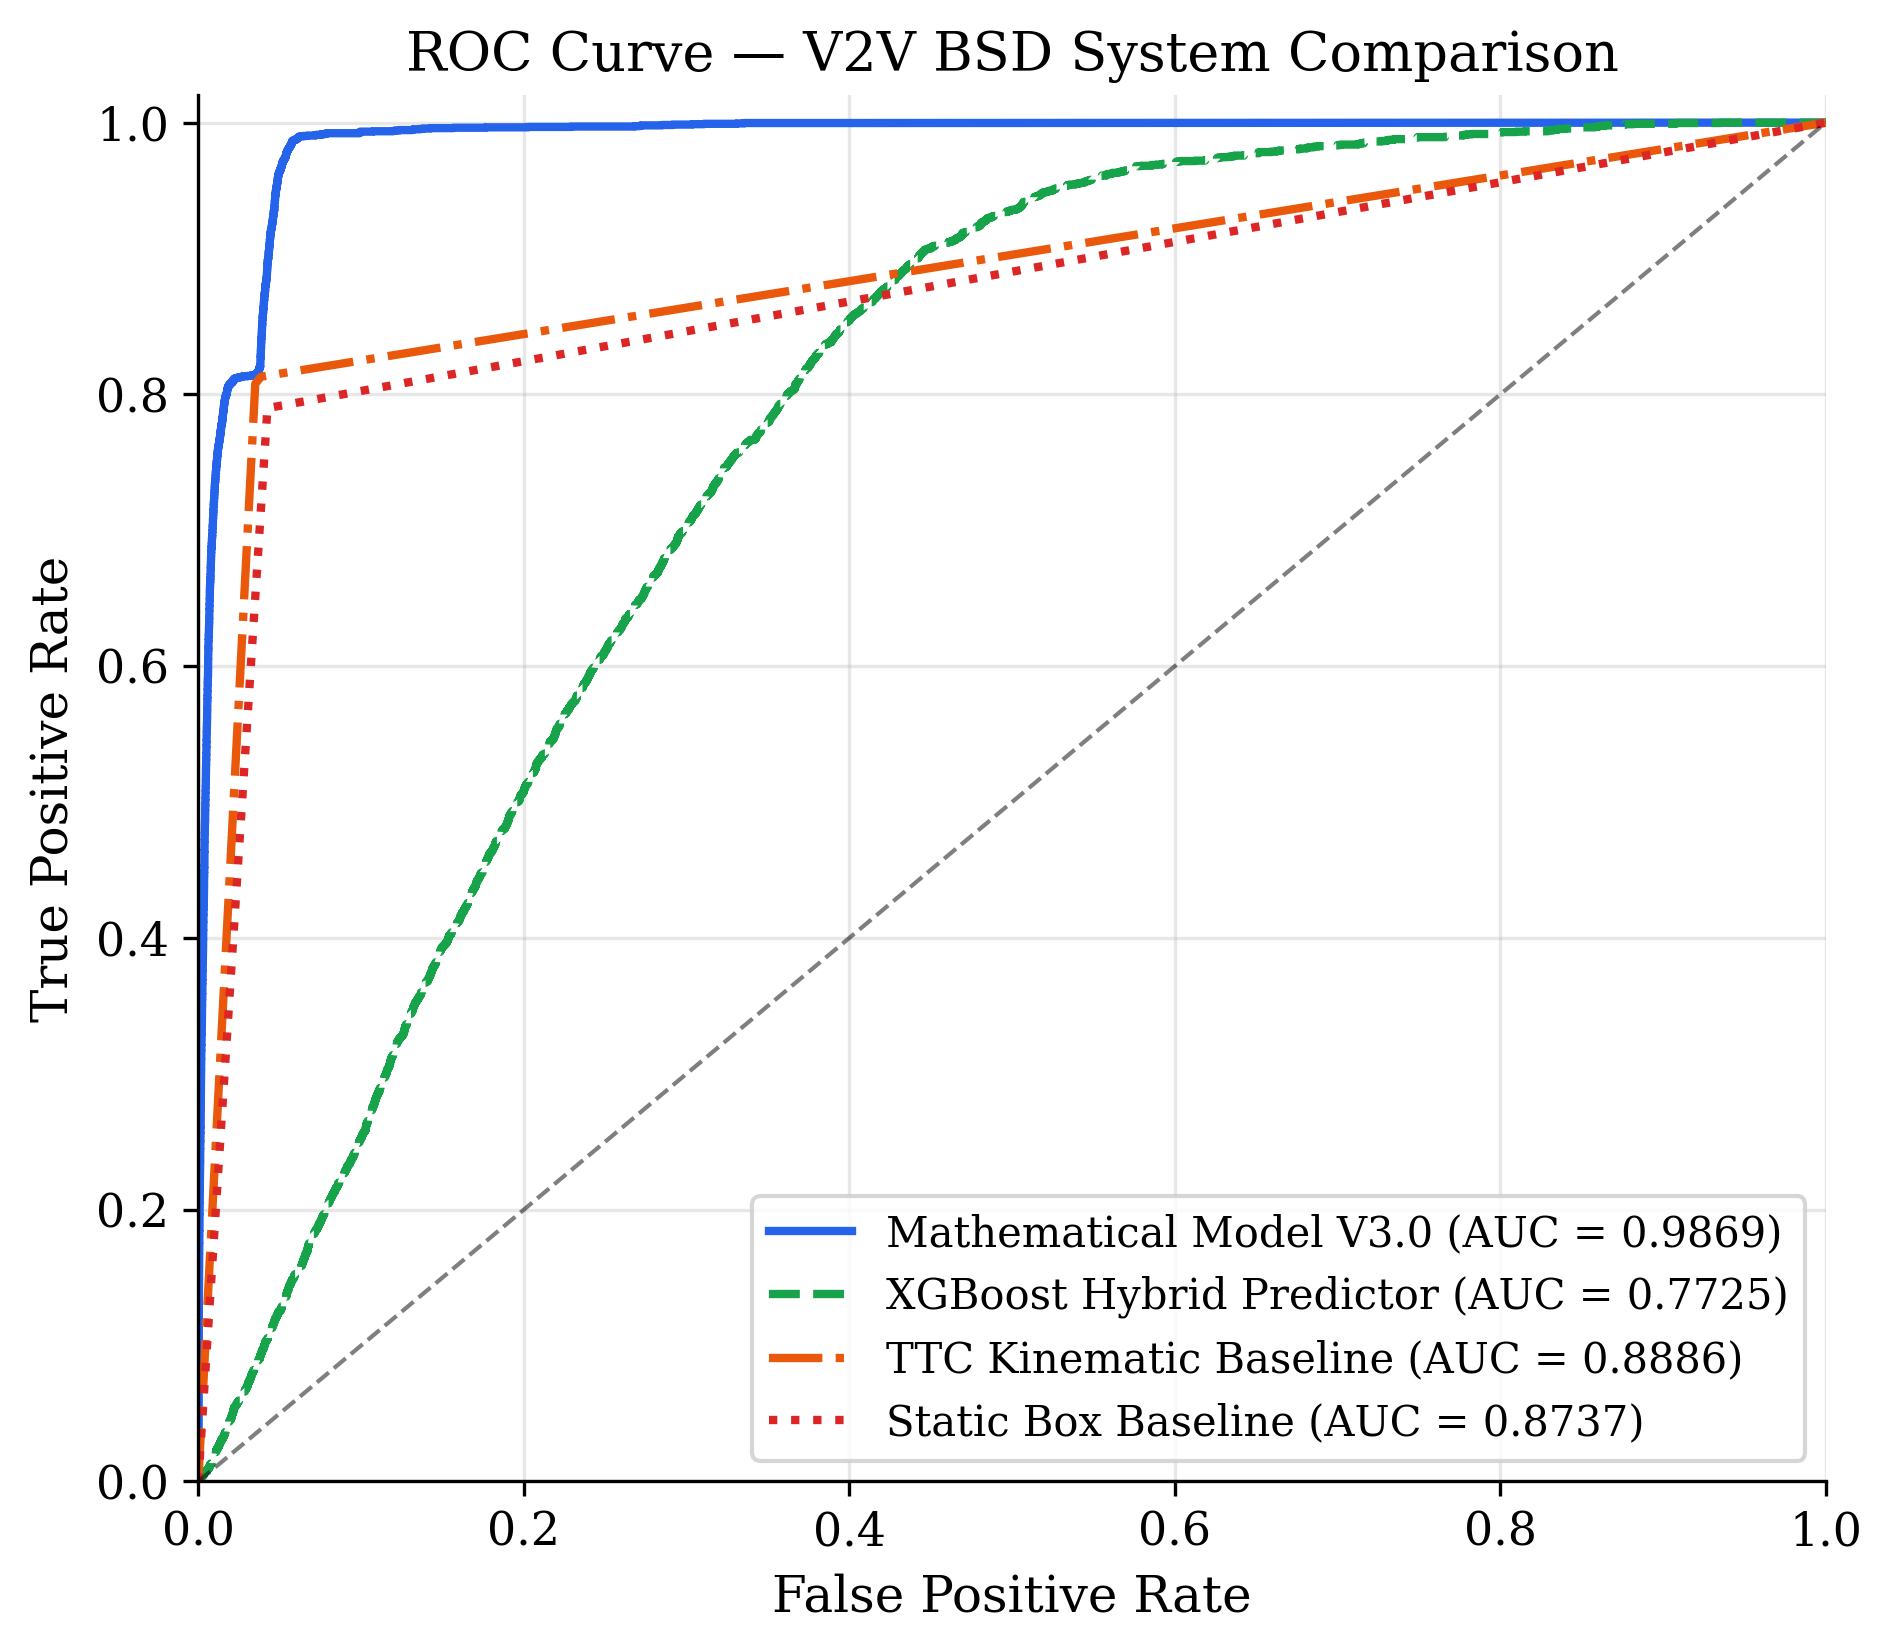
\includegraphics[width=\columnwidth]{fig1_roc_curve.png}
  \caption{ROC curves for four detection methods.}
  \label{fig:roc}
\end{figure}

\begin{figure}[htbp]
  \centering
  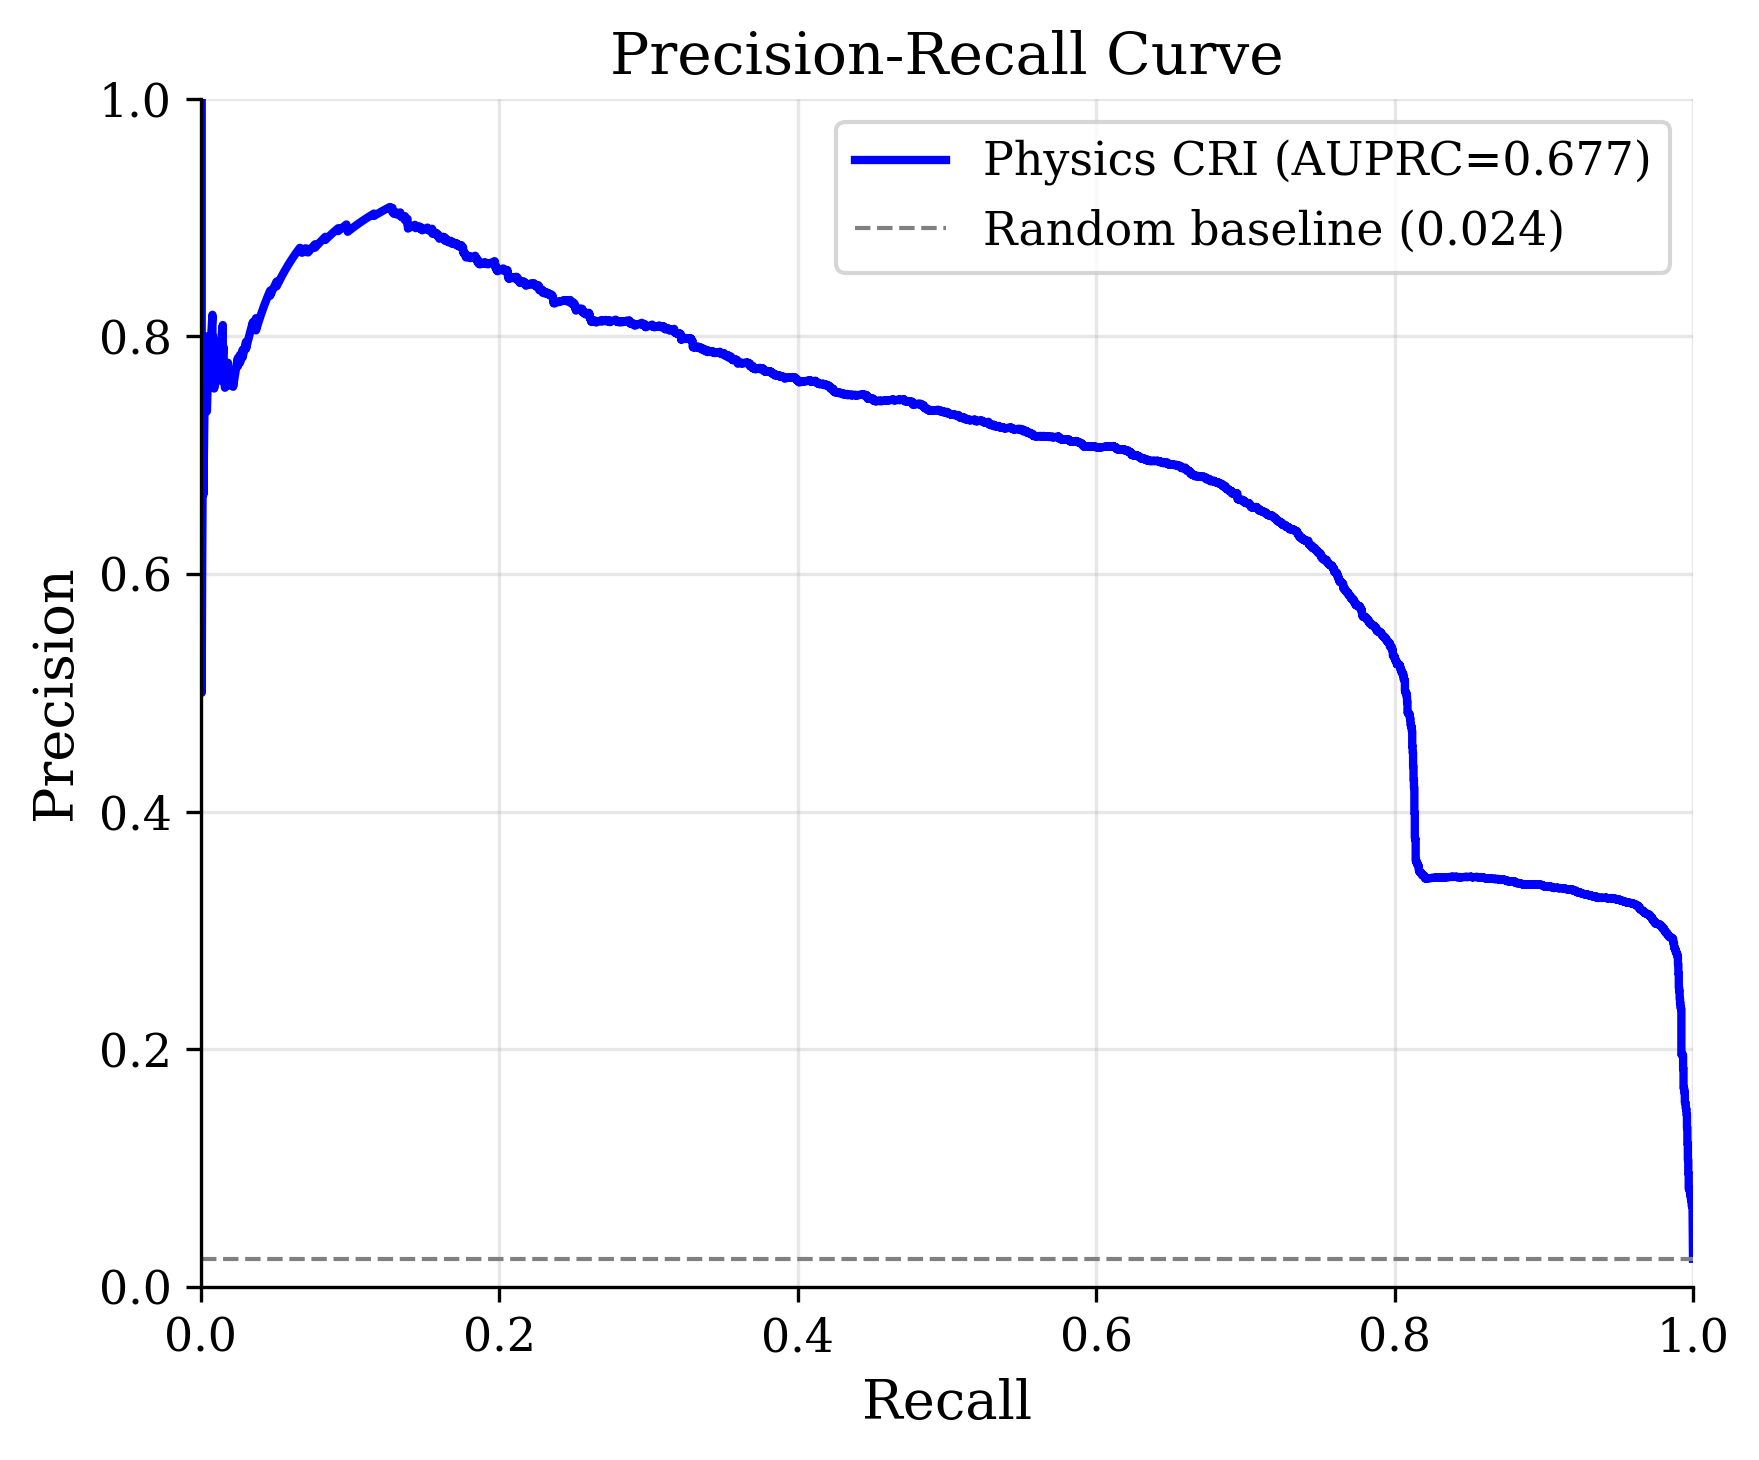
\includegraphics[width=\columnwidth]{fig9_pr_curve.png}
  \caption{Precision-Recall curve (AUPRC=0.677 vs.\ 0.024 random baseline).}
  \label{fig:pr}
\end{figure}

\subsection{Exploratory AI Model Results}
The XGBoost classifier is included as an exploratory learning-based baseline --- not as a proposed deployment component. Its AUC (0.7725) falls below both the TTC kinematic baseline (0.8886) and the static box baseline (0.8737), demonstrating that data-driven models struggle when dangerous events are extremely rare: only 54 CRITICAL samples exist in 146,051 observations. Table~\ref{tab:ai_perf} shows per-class performance. The model detects CAUTION (65\% recall) and WARNING (57\% recall) events, but fails entirely on the CRITICAL class (0\% recall, 13 test samples). This failure is systematic: cross-validation also yields 0\% CRITICAL recall across all five folds, confirming insufficient training data rather than a statistical anomaly. The confusion matrix (Fig.~\ref{fig:confusion}) visualizes this pattern.

Feature importance analysis (Fig.~\ref{fig:feat_imp}) shows that the most important features are braking dynamics (decel=0.34) and gap distance (max\_gap=0.14). The 15 input features include four perfectly correlated pairs (speed/speed\_kmh, rel\_speed/closing\_speed, accel/abs\_accel, decel/is\_braking), as shown in the correlation heatmap (Fig.~\ref{fig:feat_corr}), reducing the effective feature count to approximately 11 unique signals.

\begin{table}[htbp]
  \caption{AI Model Class Performance}
  \label{tab:ai_perf}
  \renewcommand{\arraystretch}{1.2}
  \begin{tabular}{@{}lcccc@{}}
    \toprule
    \textbf{Class} & \textbf{Prec.} & \textbf{Recall} & \textbf{F1} & \textbf{Support} \\
    \midrule
    SAFE     & 0.99 & 0.82 & 0.90 & 35,047 \\
    CAUTION  & 0.12 & 0.65 & 0.20 & 907    \\
    WARNING  & 0.11 & 0.57 & 0.18 & 546    \\
    CRITICAL & 0.00 & 0.00 & 0.00 & 13     \\
    \bottomrule
  \end{tabular}
\end{table}

\begin{figure}[htbp]
  \centering
  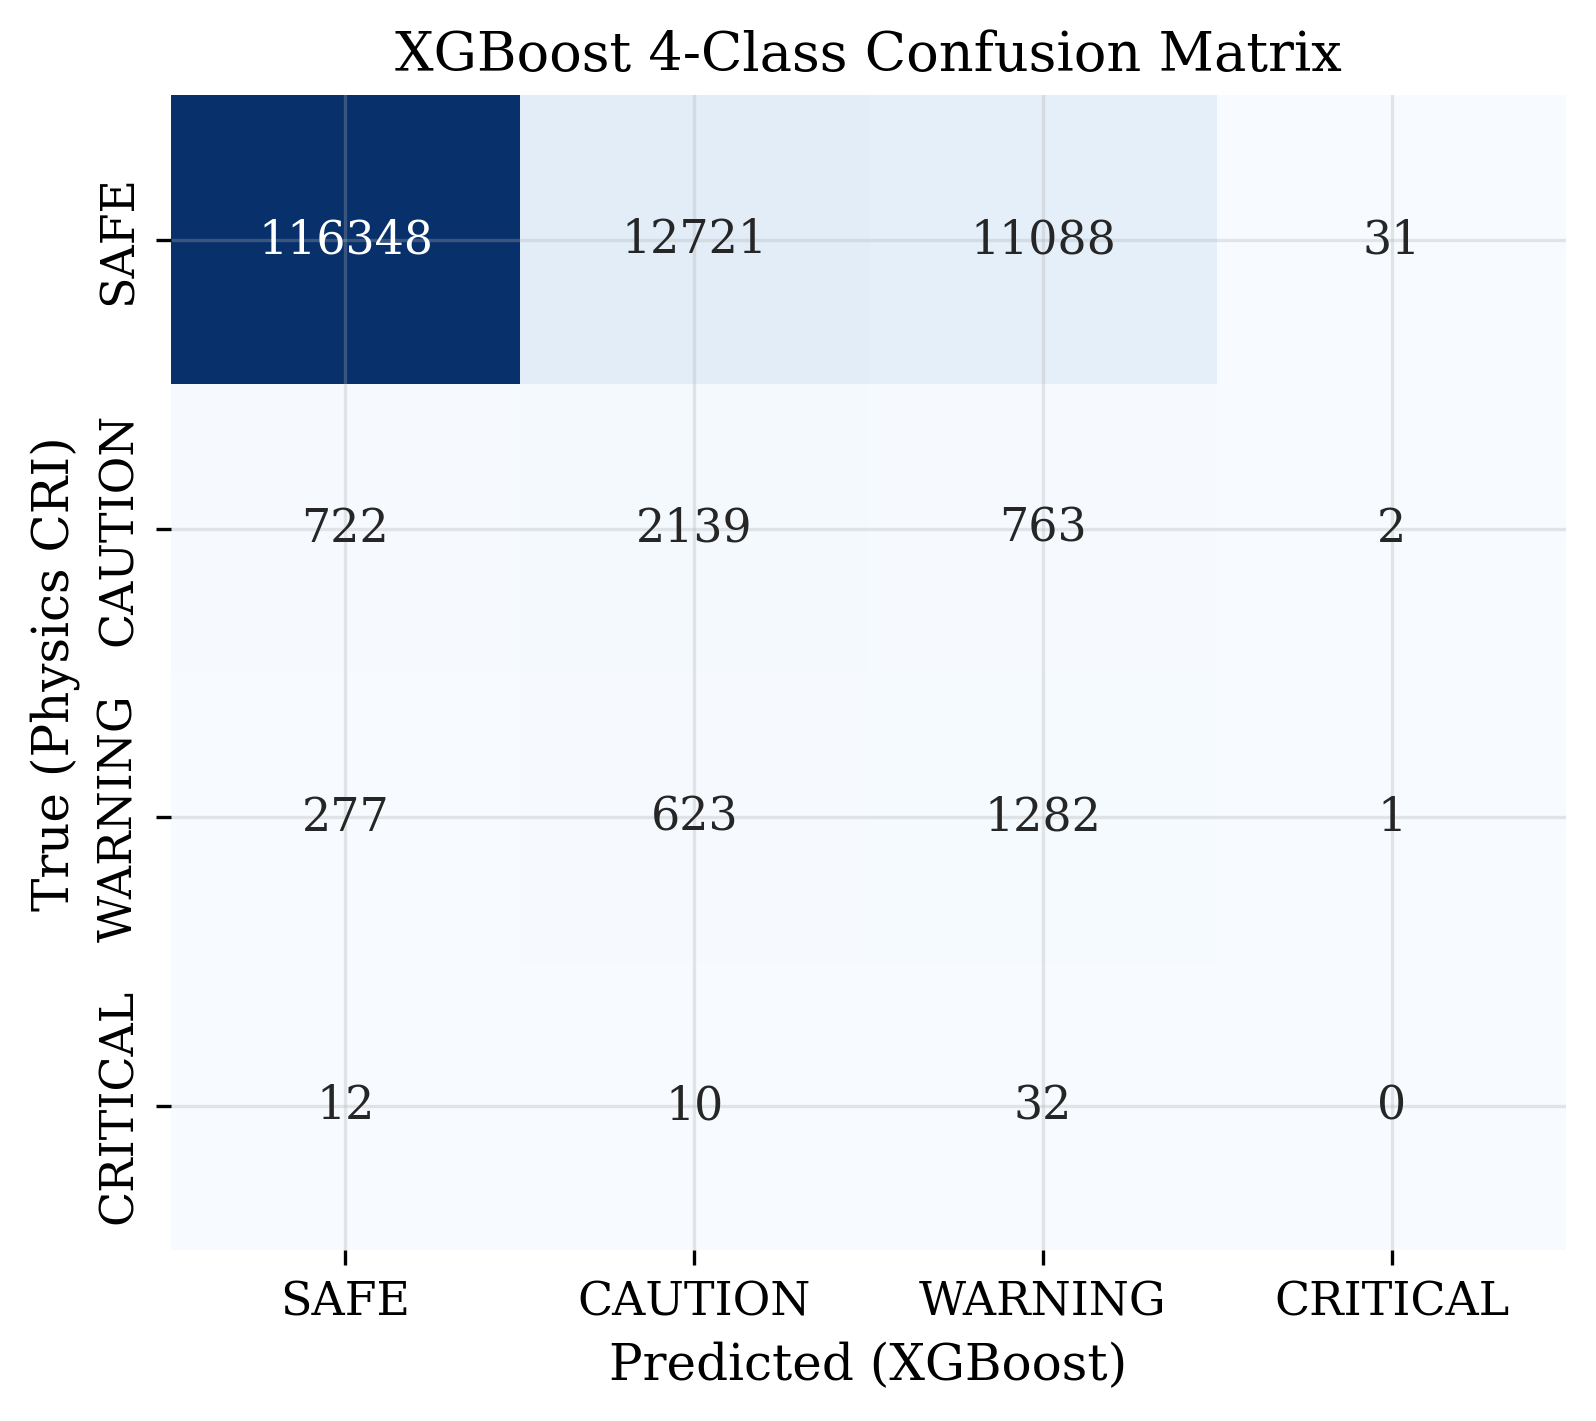
\includegraphics[width=\columnwidth]{fig7_confusion_matrix.png}
  \caption{Four-class confusion matrix: XGBoost predictions vs.\ physics-model CRI labels. CRITICAL detection fails due to extreme class rarity (54 total samples).}
  \label{fig:confusion}
\end{figure}

\begin{figure}[htbp]
  \centering
  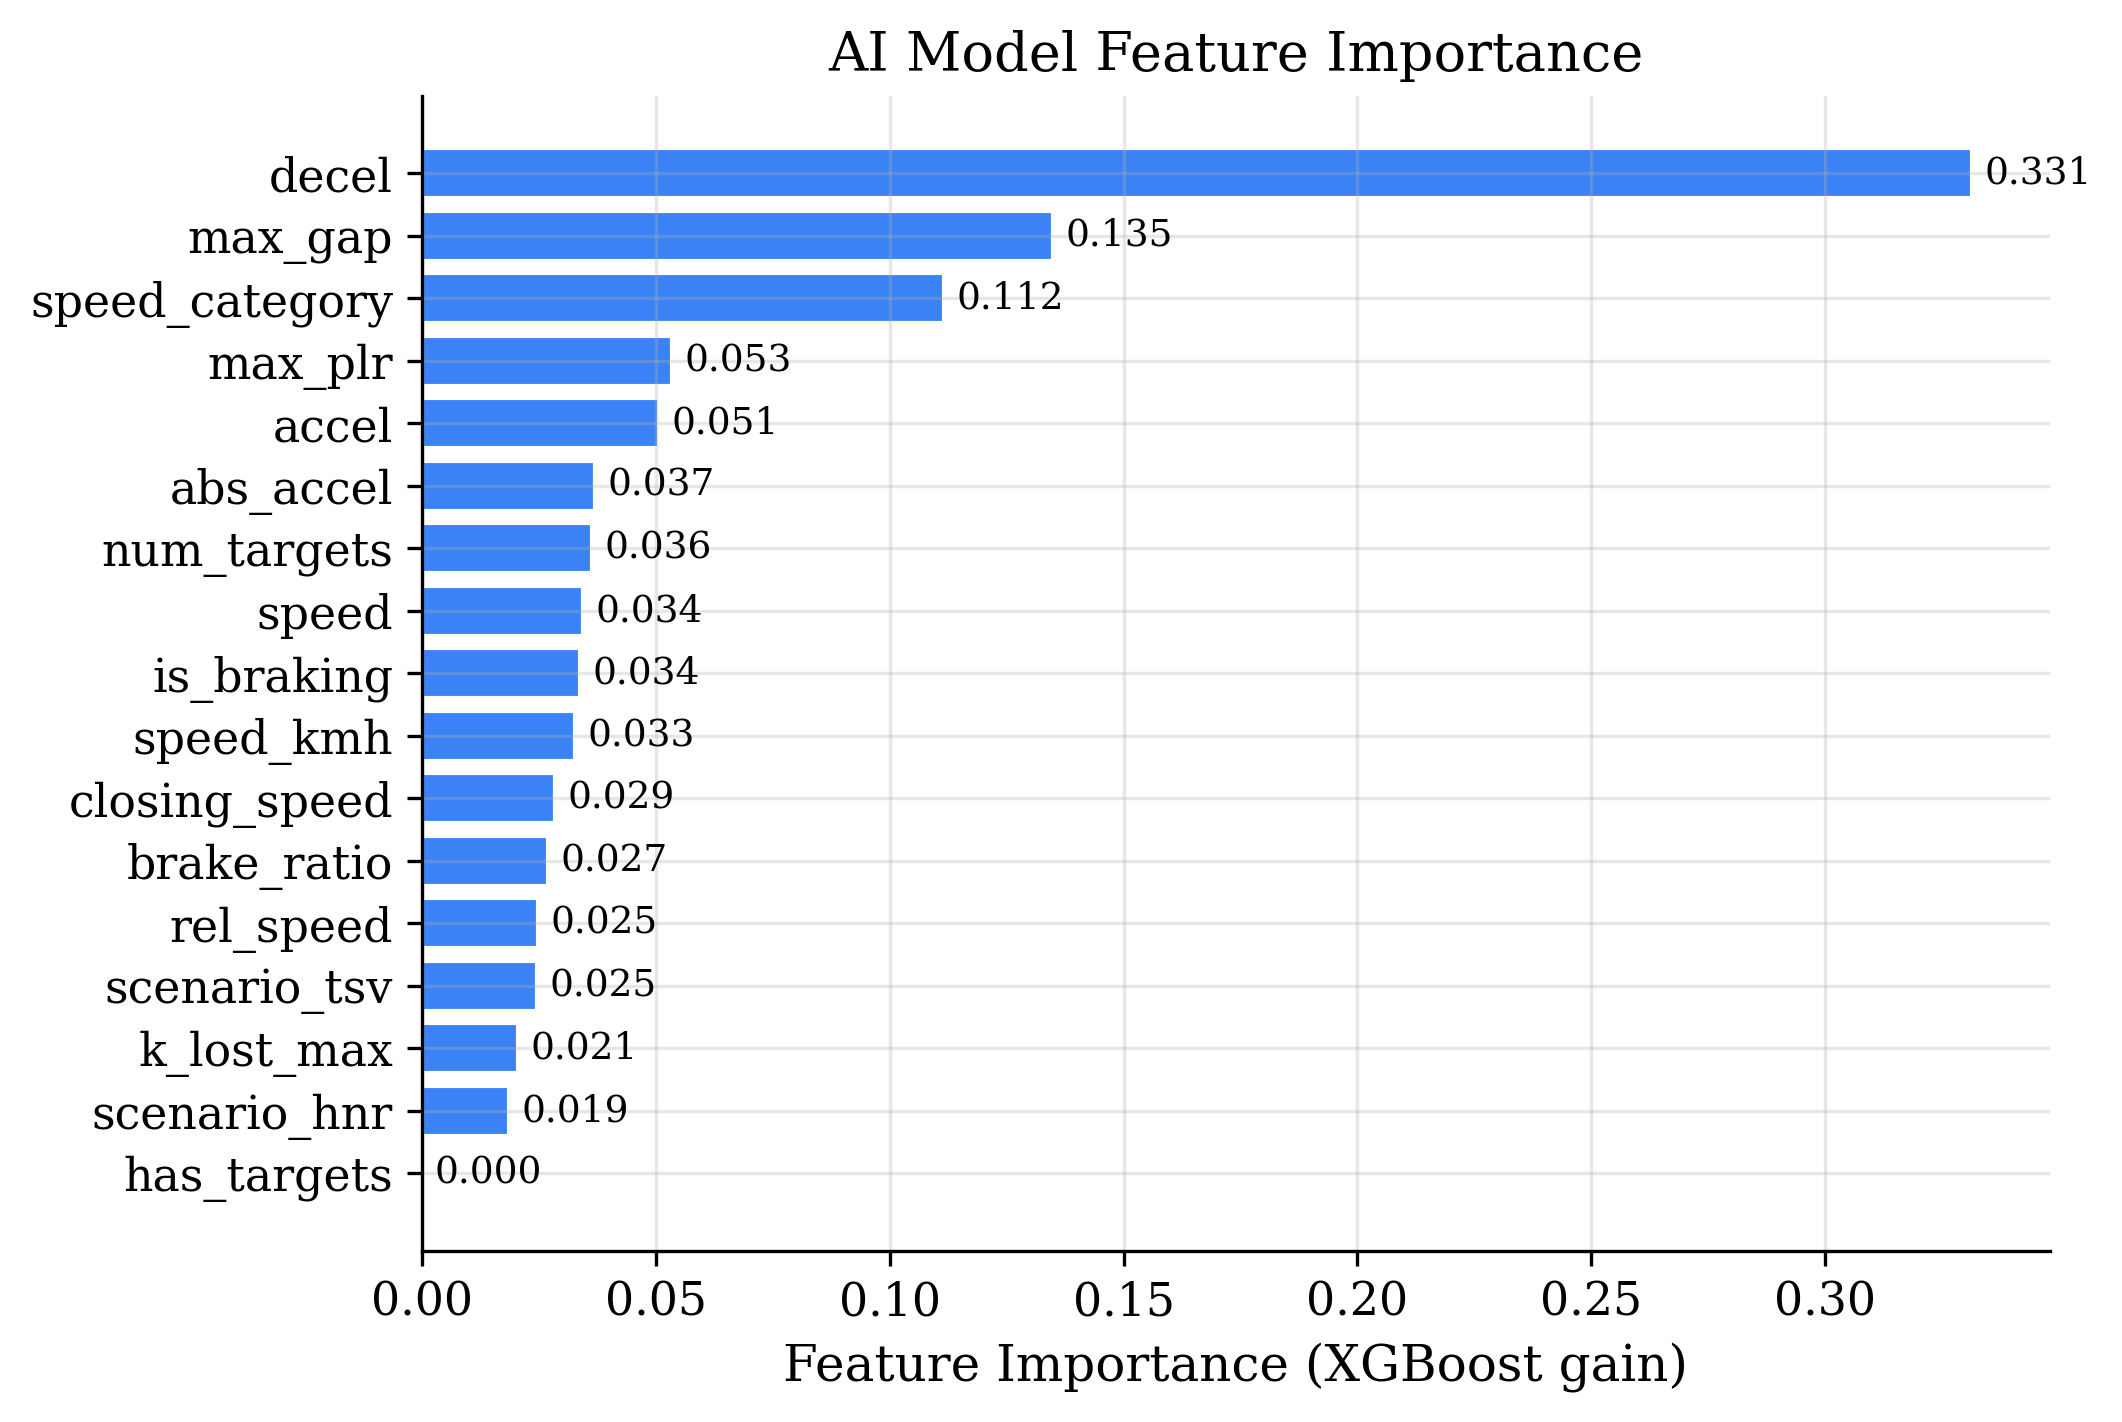
\includegraphics[width=\columnwidth]{fig3_feature_importance.png}
  \caption{XGBoost feature importance (15 features). Deceleration and gap distance dominate. Scenario labels are excluded from the feature set.}
  \label{fig:feat_imp}
\end{figure}

\begin{figure}[htbp]
  \centering
  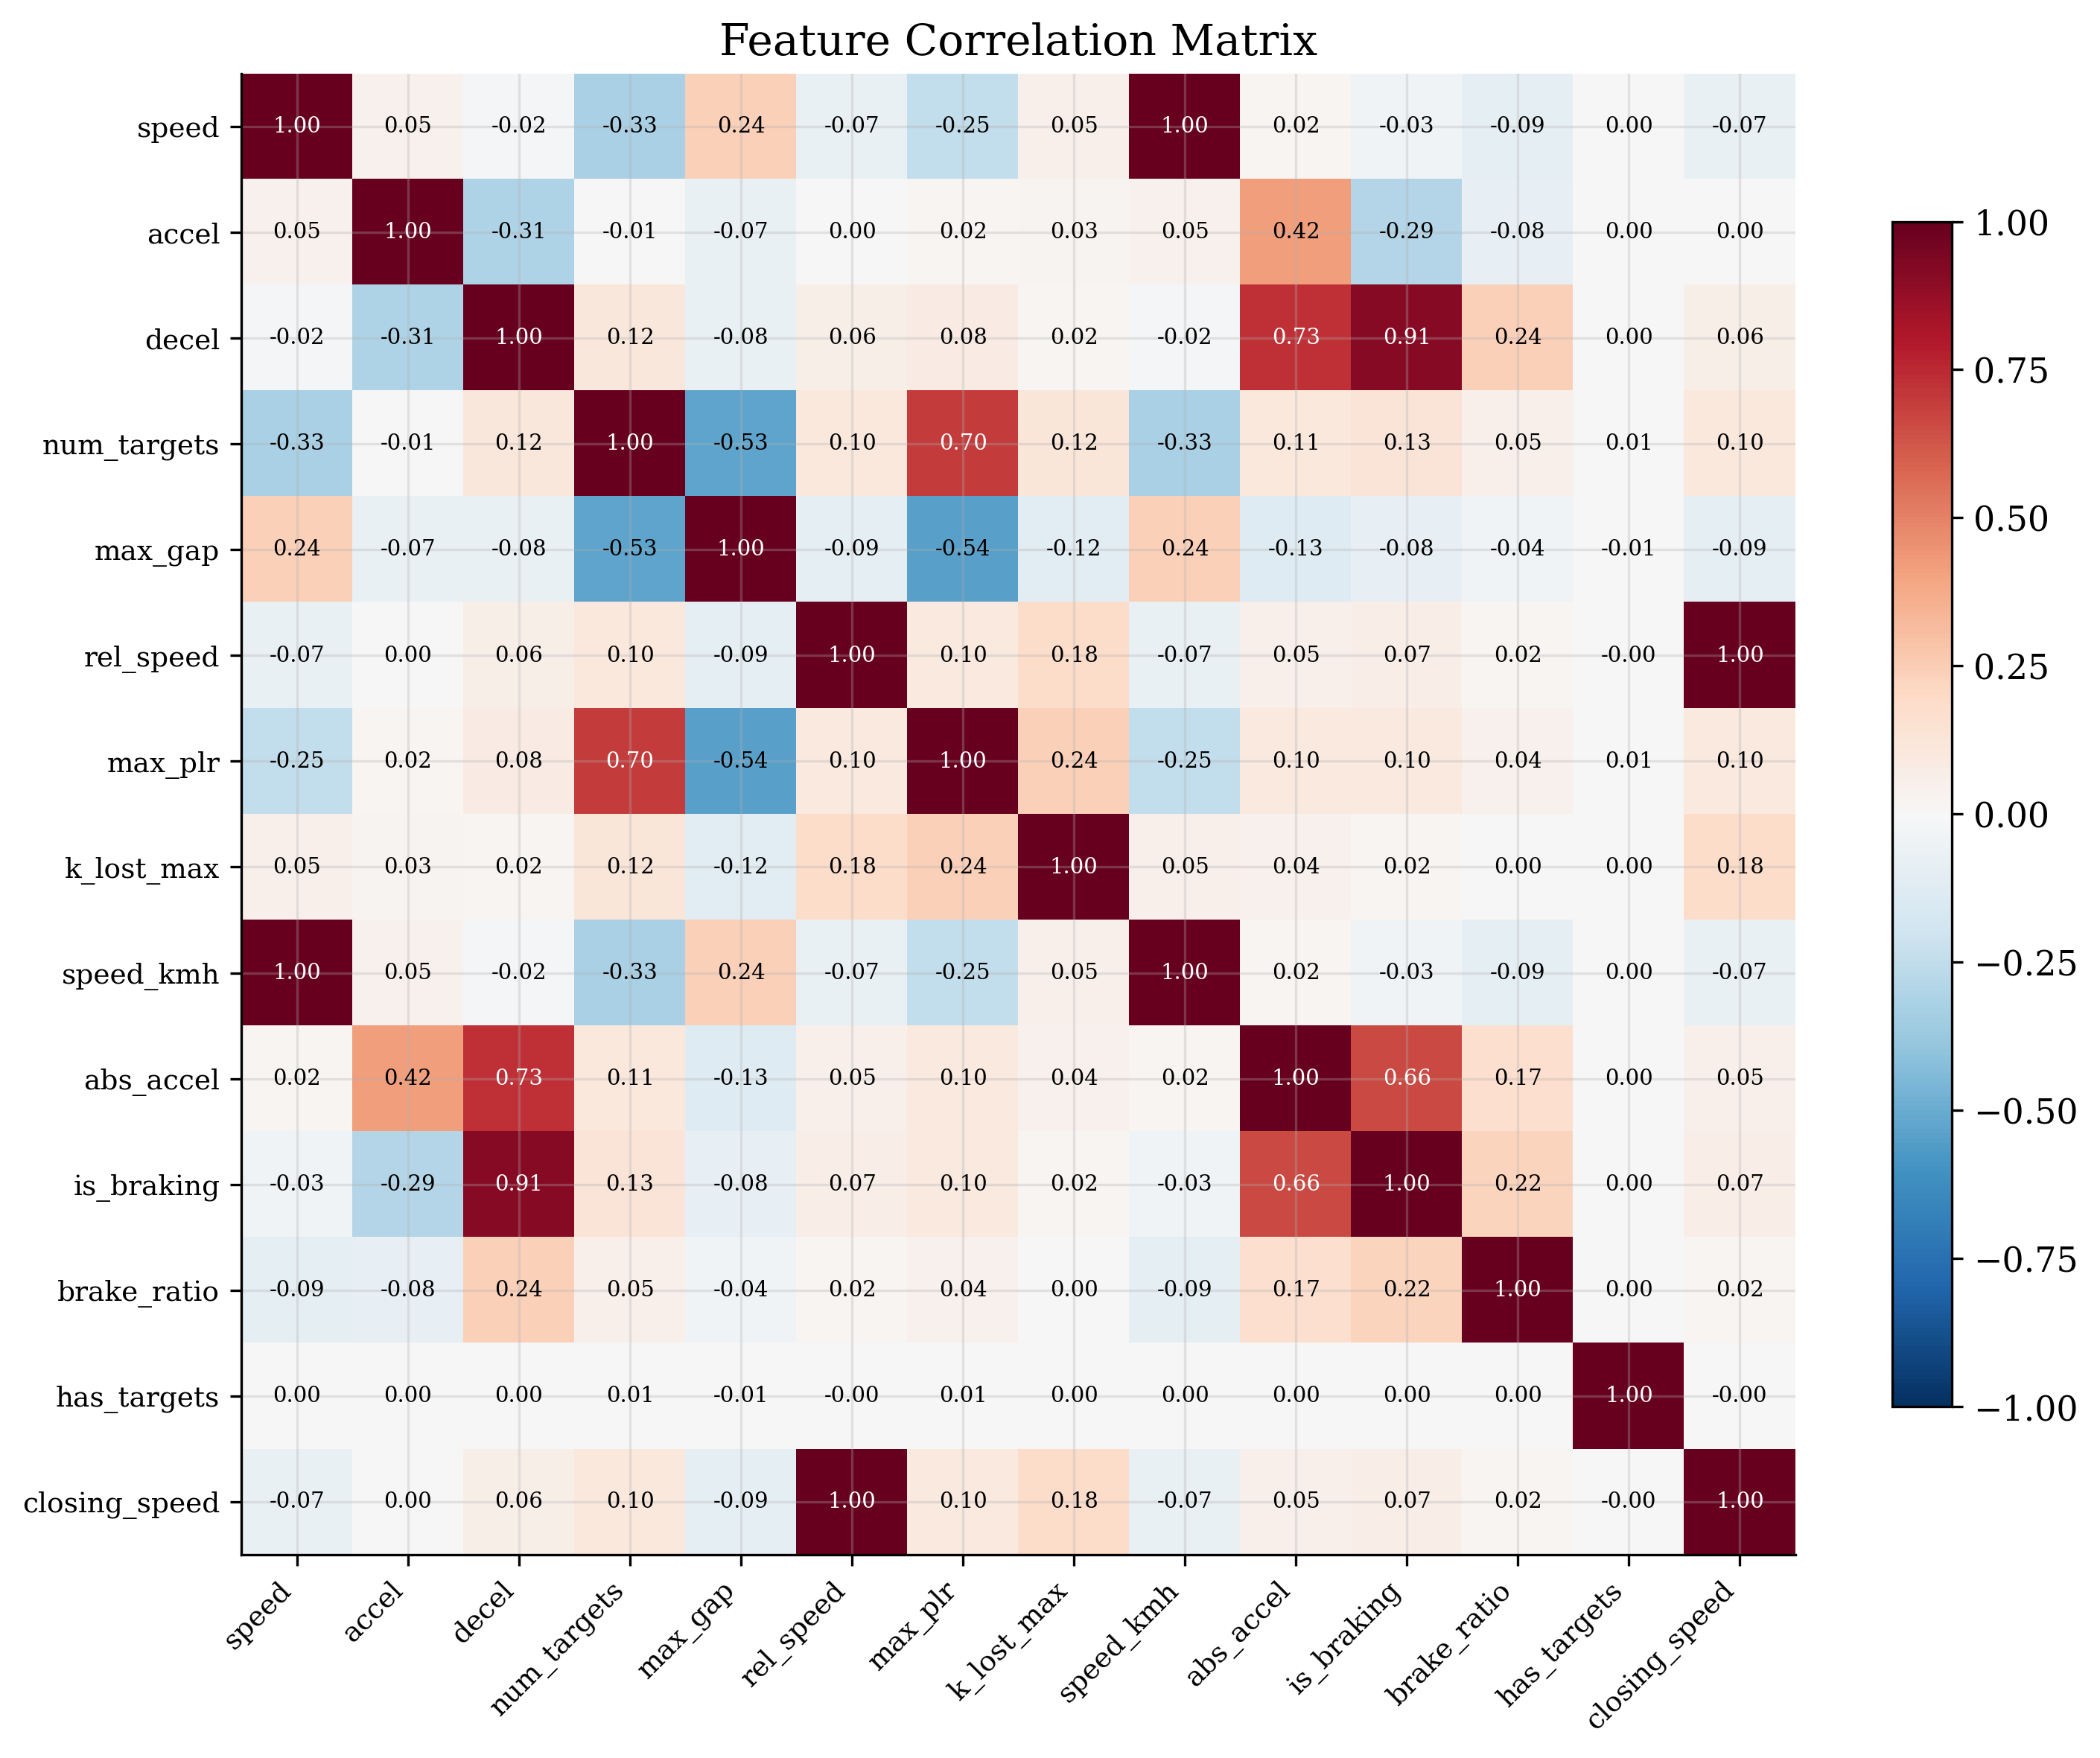
\includegraphics[width=\columnwidth]{fig12_feature_correlation.png}
  \caption{Feature correlation heatmap. Notable redundancies include speed/speed\_kmh ($r=1.0$) and rel\_speed/closing\_speed ($r=1.0$), suggesting potential for feature set reduction.}
  \label{fig:feat_corr}
\end{figure}

\subsection{Per-Scenario Performance}
To verify the system works across different hazard types, AUC was computed separately for each scenario (Table~\ref{tab:scenario_auc}). The narrow spread ($\Delta$AUC~$<$~0.002) confirms the system is robust across different traffic conditions.

Fig.~\ref{fig:speed_cri} shows the relationship between ego vehicle speed and CRI across scenarios. Higher speeds generally produce higher CRI values, with HNR scenarios showing elevated risk at lower speeds due to reduced friction. Fig.~\ref{fig:calibration} shows the calibration plot, assessing whether CRI scores correspond to actual danger frequencies.

\subsection{Multi-Seed Robustness}
To confirm results are not dependent on a single random traffic pattern, the simulation was repeated with six random seeds: the primary seed~42 (used throughout this paper) plus five additional seeds (Table~\ref{tab:multiseed}). Seed~42 produces the most challenging traffic mix (highest proportion of dense interactions near the Atal Bridge merge zones), which accounts for its slightly lower AUC. All results reported in prior sections use seed~42 as the conservative baseline.

\begin{table}[htbp]
  \caption{Per-Scenario AUC (Physics Model)}
  \label{tab:scenario_auc}
  \renewcommand{\arraystretch}{1.2}
  \begin{tabular}{@{}lccc@{}}
    \toprule
    \textbf{Scenario} & \textbf{AUC} & \textbf{$n$} & \textbf{Positives} \\
    \midrule
    Normal traffic & 0.9874 & 72,494 & 1,619 \\
    TSV            & 0.9877 & 28,246 & 653   \\
    HNR            & 0.9857 & 45,311 & 1,193 \\
    \bottomrule
  \end{tabular}
\end{table}

\begin{table}[htbp]
  \caption{Multi-Seed Results ($N=6$)}
  \label{tab:multiseed}
  \renewcommand{\arraystretch}{1.2}
  \begin{tabular}{@{}lcc@{}}
    \toprule
    \textbf{Metric} & \textbf{Physics (V3.0)} & \textbf{XGBoost} \\
    \midrule
    Seed 42 (primary)   & 0.9869 & 0.7725 \\
    Seeds 10--50 (mean) & $0.9971 \pm 0.0007$ & $0.8985 \pm 0.0095$ \\
    \textbf{All 6 seeds} & $\mathbf{0.9954 \pm 0.0041}$ & $0.8775 \pm 0.0520$ \\
    \bottomrule
  \end{tabular}
\end{table}

\begin{figure}[htbp]
  \centering
  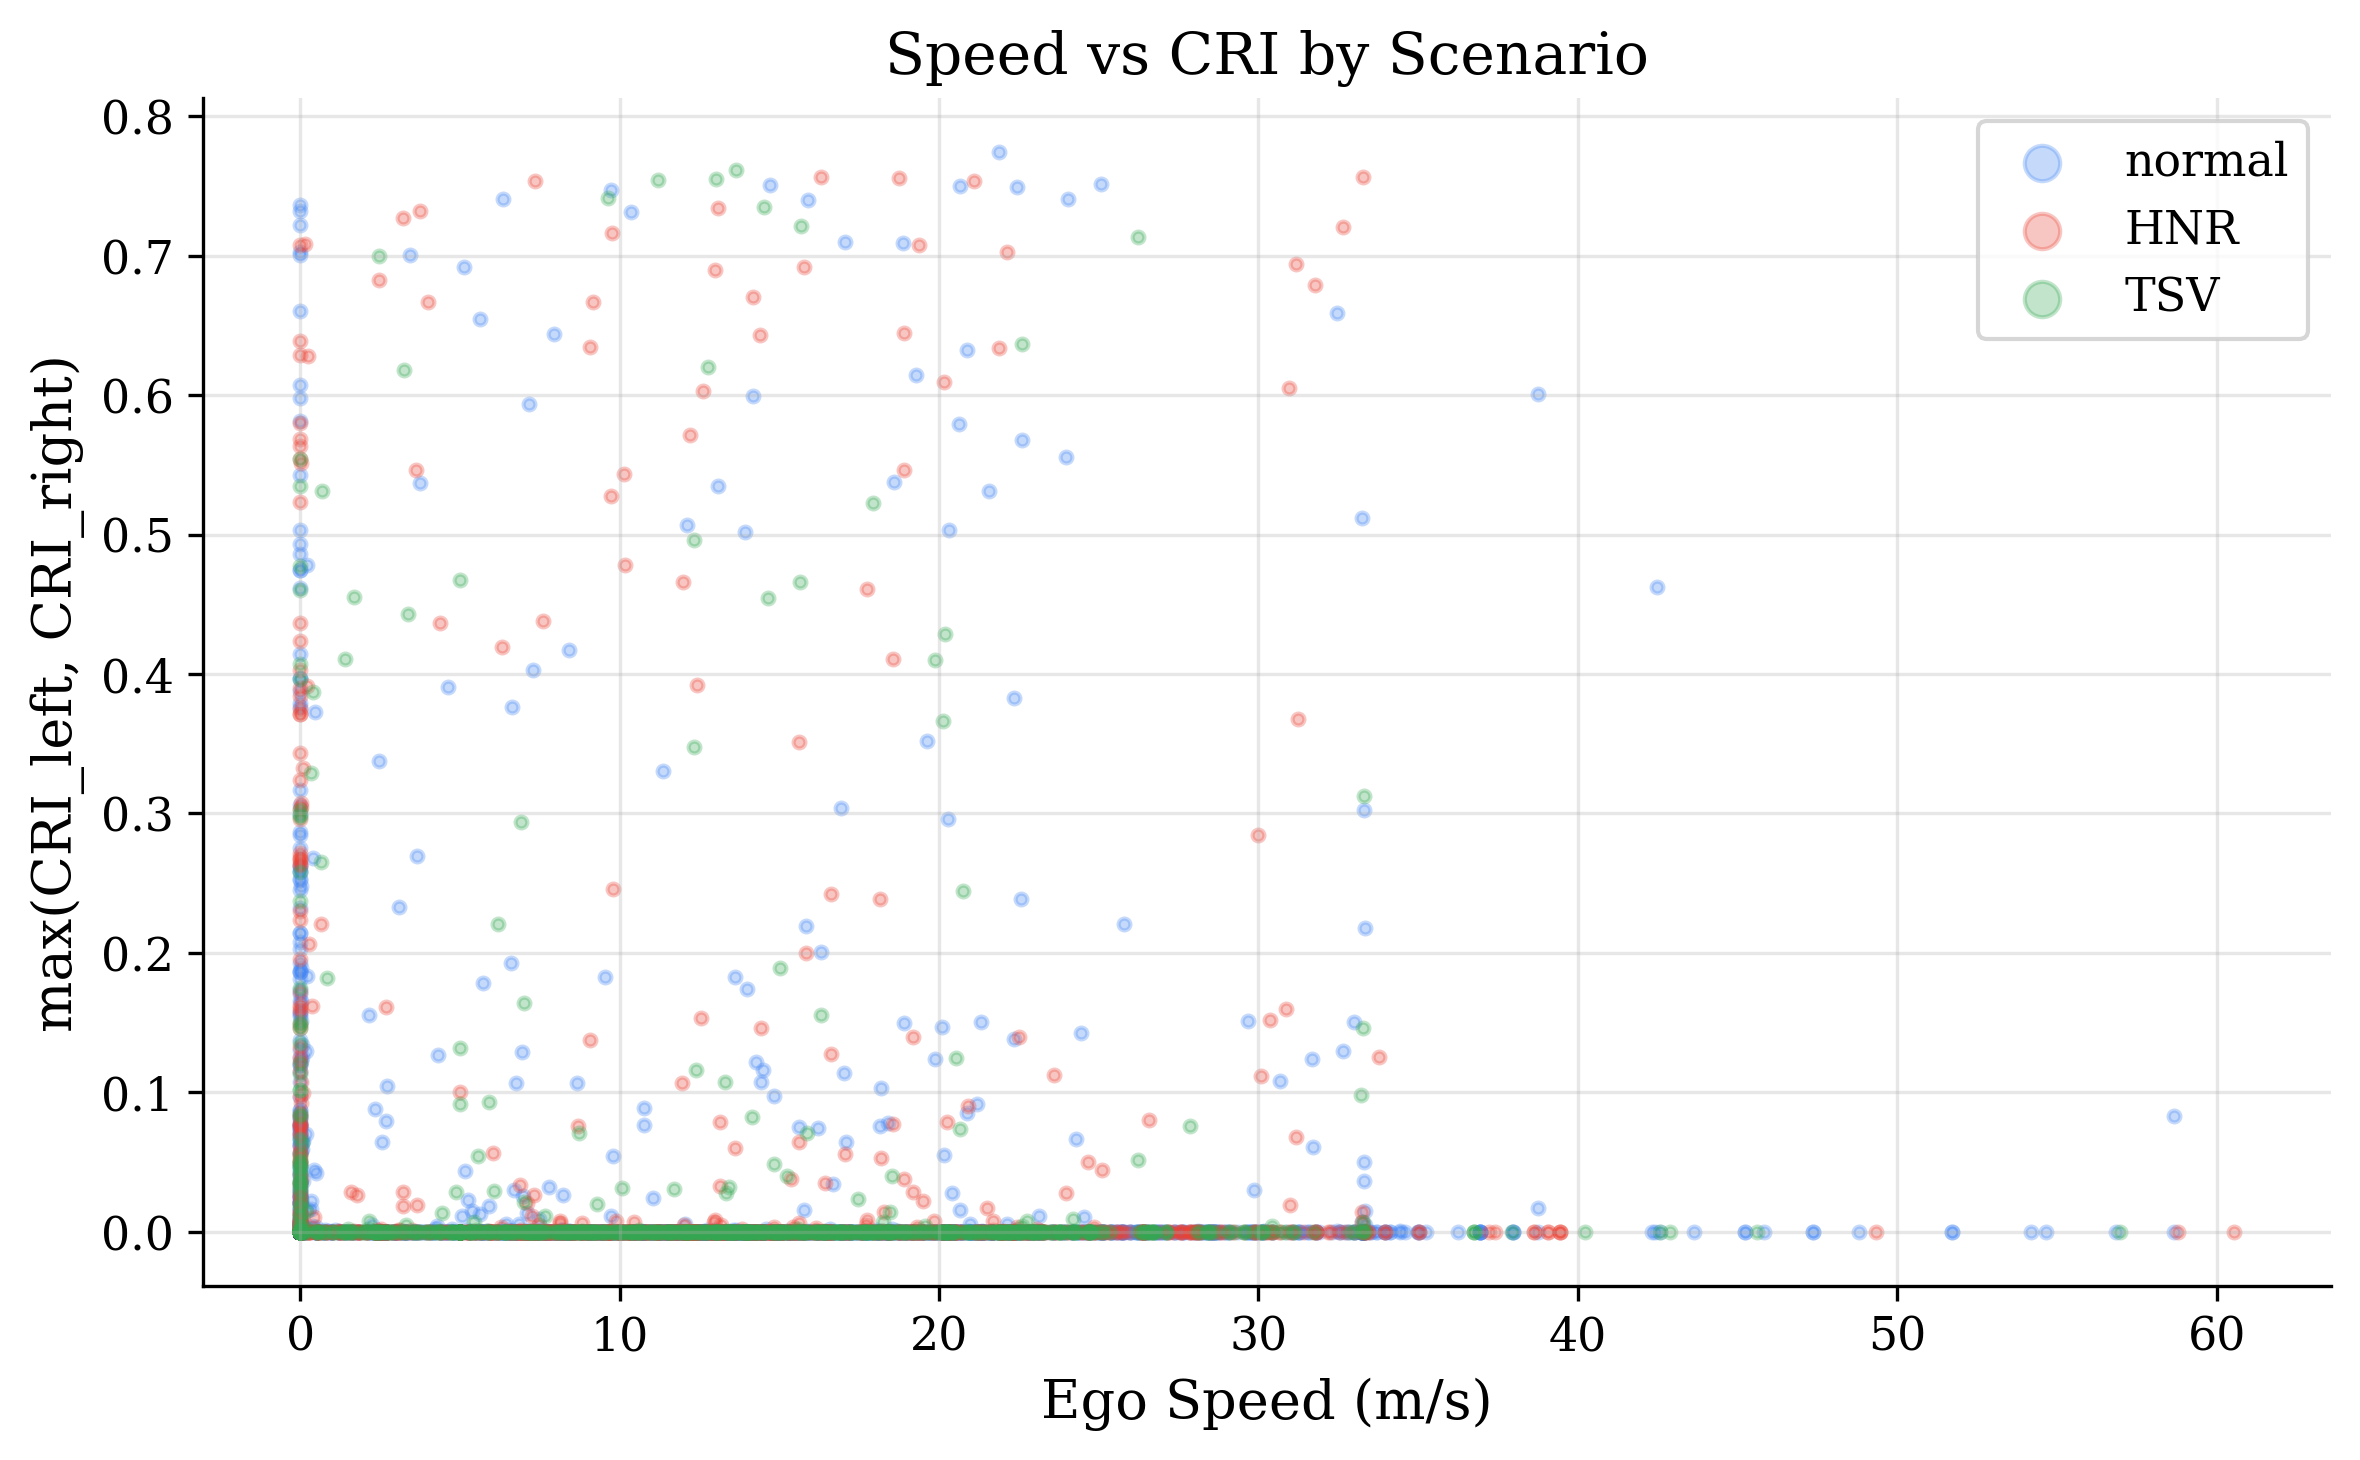
\includegraphics[width=\columnwidth]{fig13_speed_cri_scatter.png}
  \caption{Ego speed vs.\ maximum CRI, colored by scenario type (5,000 sampled rows). HNR scenarios show elevated risk at lower speeds due to reduced friction and narrow lanes.}
  \label{fig:speed_cri}
\end{figure}

\begin{figure}[htbp]
  \centering
  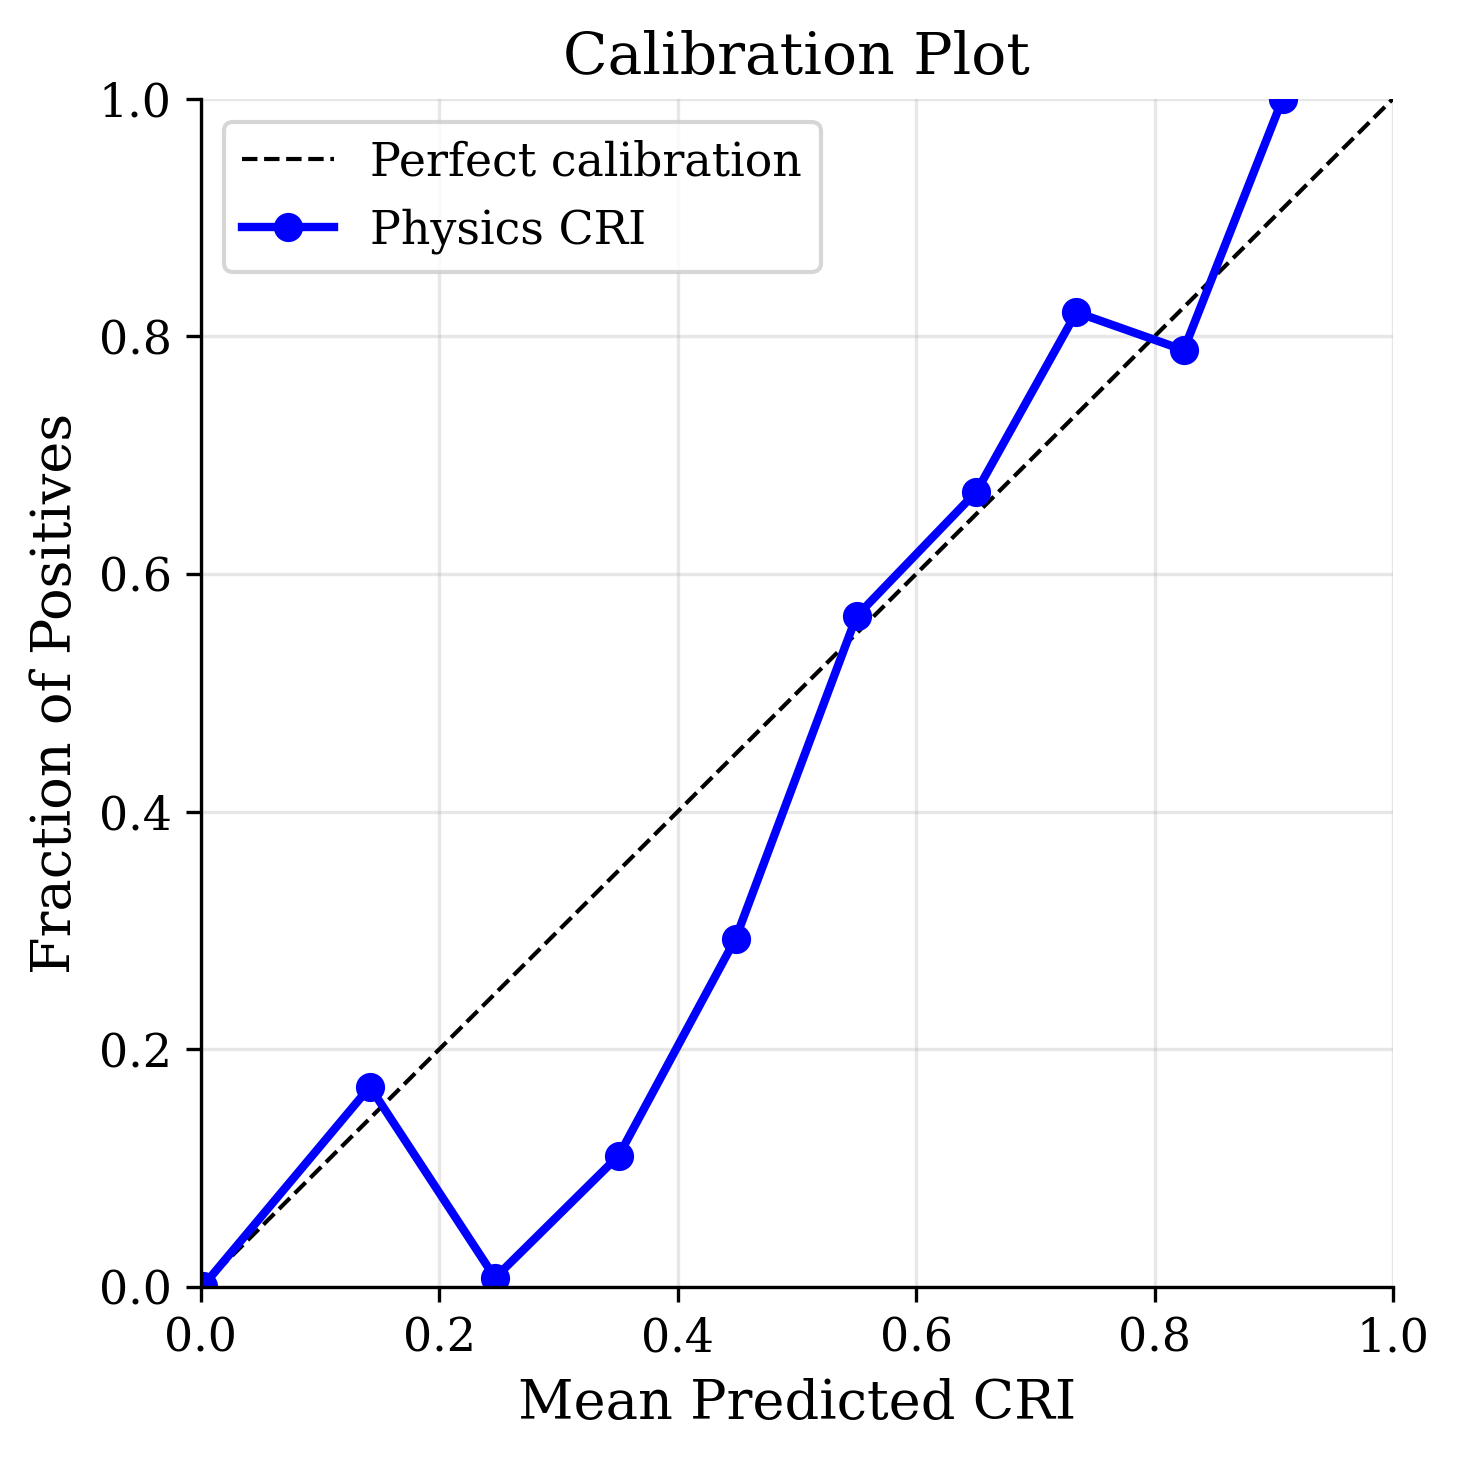
\includegraphics[width=\columnwidth]{fig11_calibration.png}
  \caption{Calibration plot: predicted CRI vs.\ observed positive fraction. The proxy ground truth uses kinematic near-miss events (2.37\% positive rate).}
  \label{fig:calibration}
\end{figure}

\subsection{Ablation Study}
Five configurations were tested (Table~\ref{tab:ablation}). Including intent ($\gamma=0.20$, A3/A4) without turn signals causes 44\% F1 drop, validating $\gamma=0$. A5 ($\alpha{=}0.20, \beta{=}0.80$) is selected over A2 ($\alpha{=}0.50, \beta{=}0.50$) for better AUC rank-ordering (0.9869 vs.\ 0.9842) despite nearly identical single-threshold F1.

\begin{table}[htbp]
  \caption{Ablation Study Results}
  \label{tab:ablation}
  \renewcommand{\arraystretch}{1.2}
  \begin{tabular}{@{}ccccccc@{}}
    \toprule
    \textbf{Config} & $\alpha$ & $\beta$ & $\gamma$ & \textbf{Lat TTC}
      & \textbf{F1 (0.60)} & \textbf{F1 (0.80)} \\
    \midrule
    A1 & 1.00 & 0.00 & 0.00 & $\times$ & 0.652 & 0.519 \\
    A2 & 0.50 & 0.50 & 0.00 & $\times$ & 0.583 & 0.491 \\
    A3 & 0.35 & 0.45 & 0.20 & $\times$ & 0.328 & 0.216 \\
    A4 & 0.35 & 0.45 & 0.20 & $\checkmark$ & 0.328 & 0.216 \\
    \textbf{A5} & \textbf{0.20} & \textbf{0.80} & \textbf{0.00}
      & $\checkmark$ & \textbf{0.583} & \textbf{0.494} \\
    \bottomrule
  \end{tabular}
\end{table}

\subsection{Sensitivity Analysis}
The system maintains strong performance under parameter variation (Fig.~\ref{fig:sensitivity}): robust with GPS noise up to 3.0~m and packet loss up to 20\%.

\begin{figure}[htbp]
  \centering
  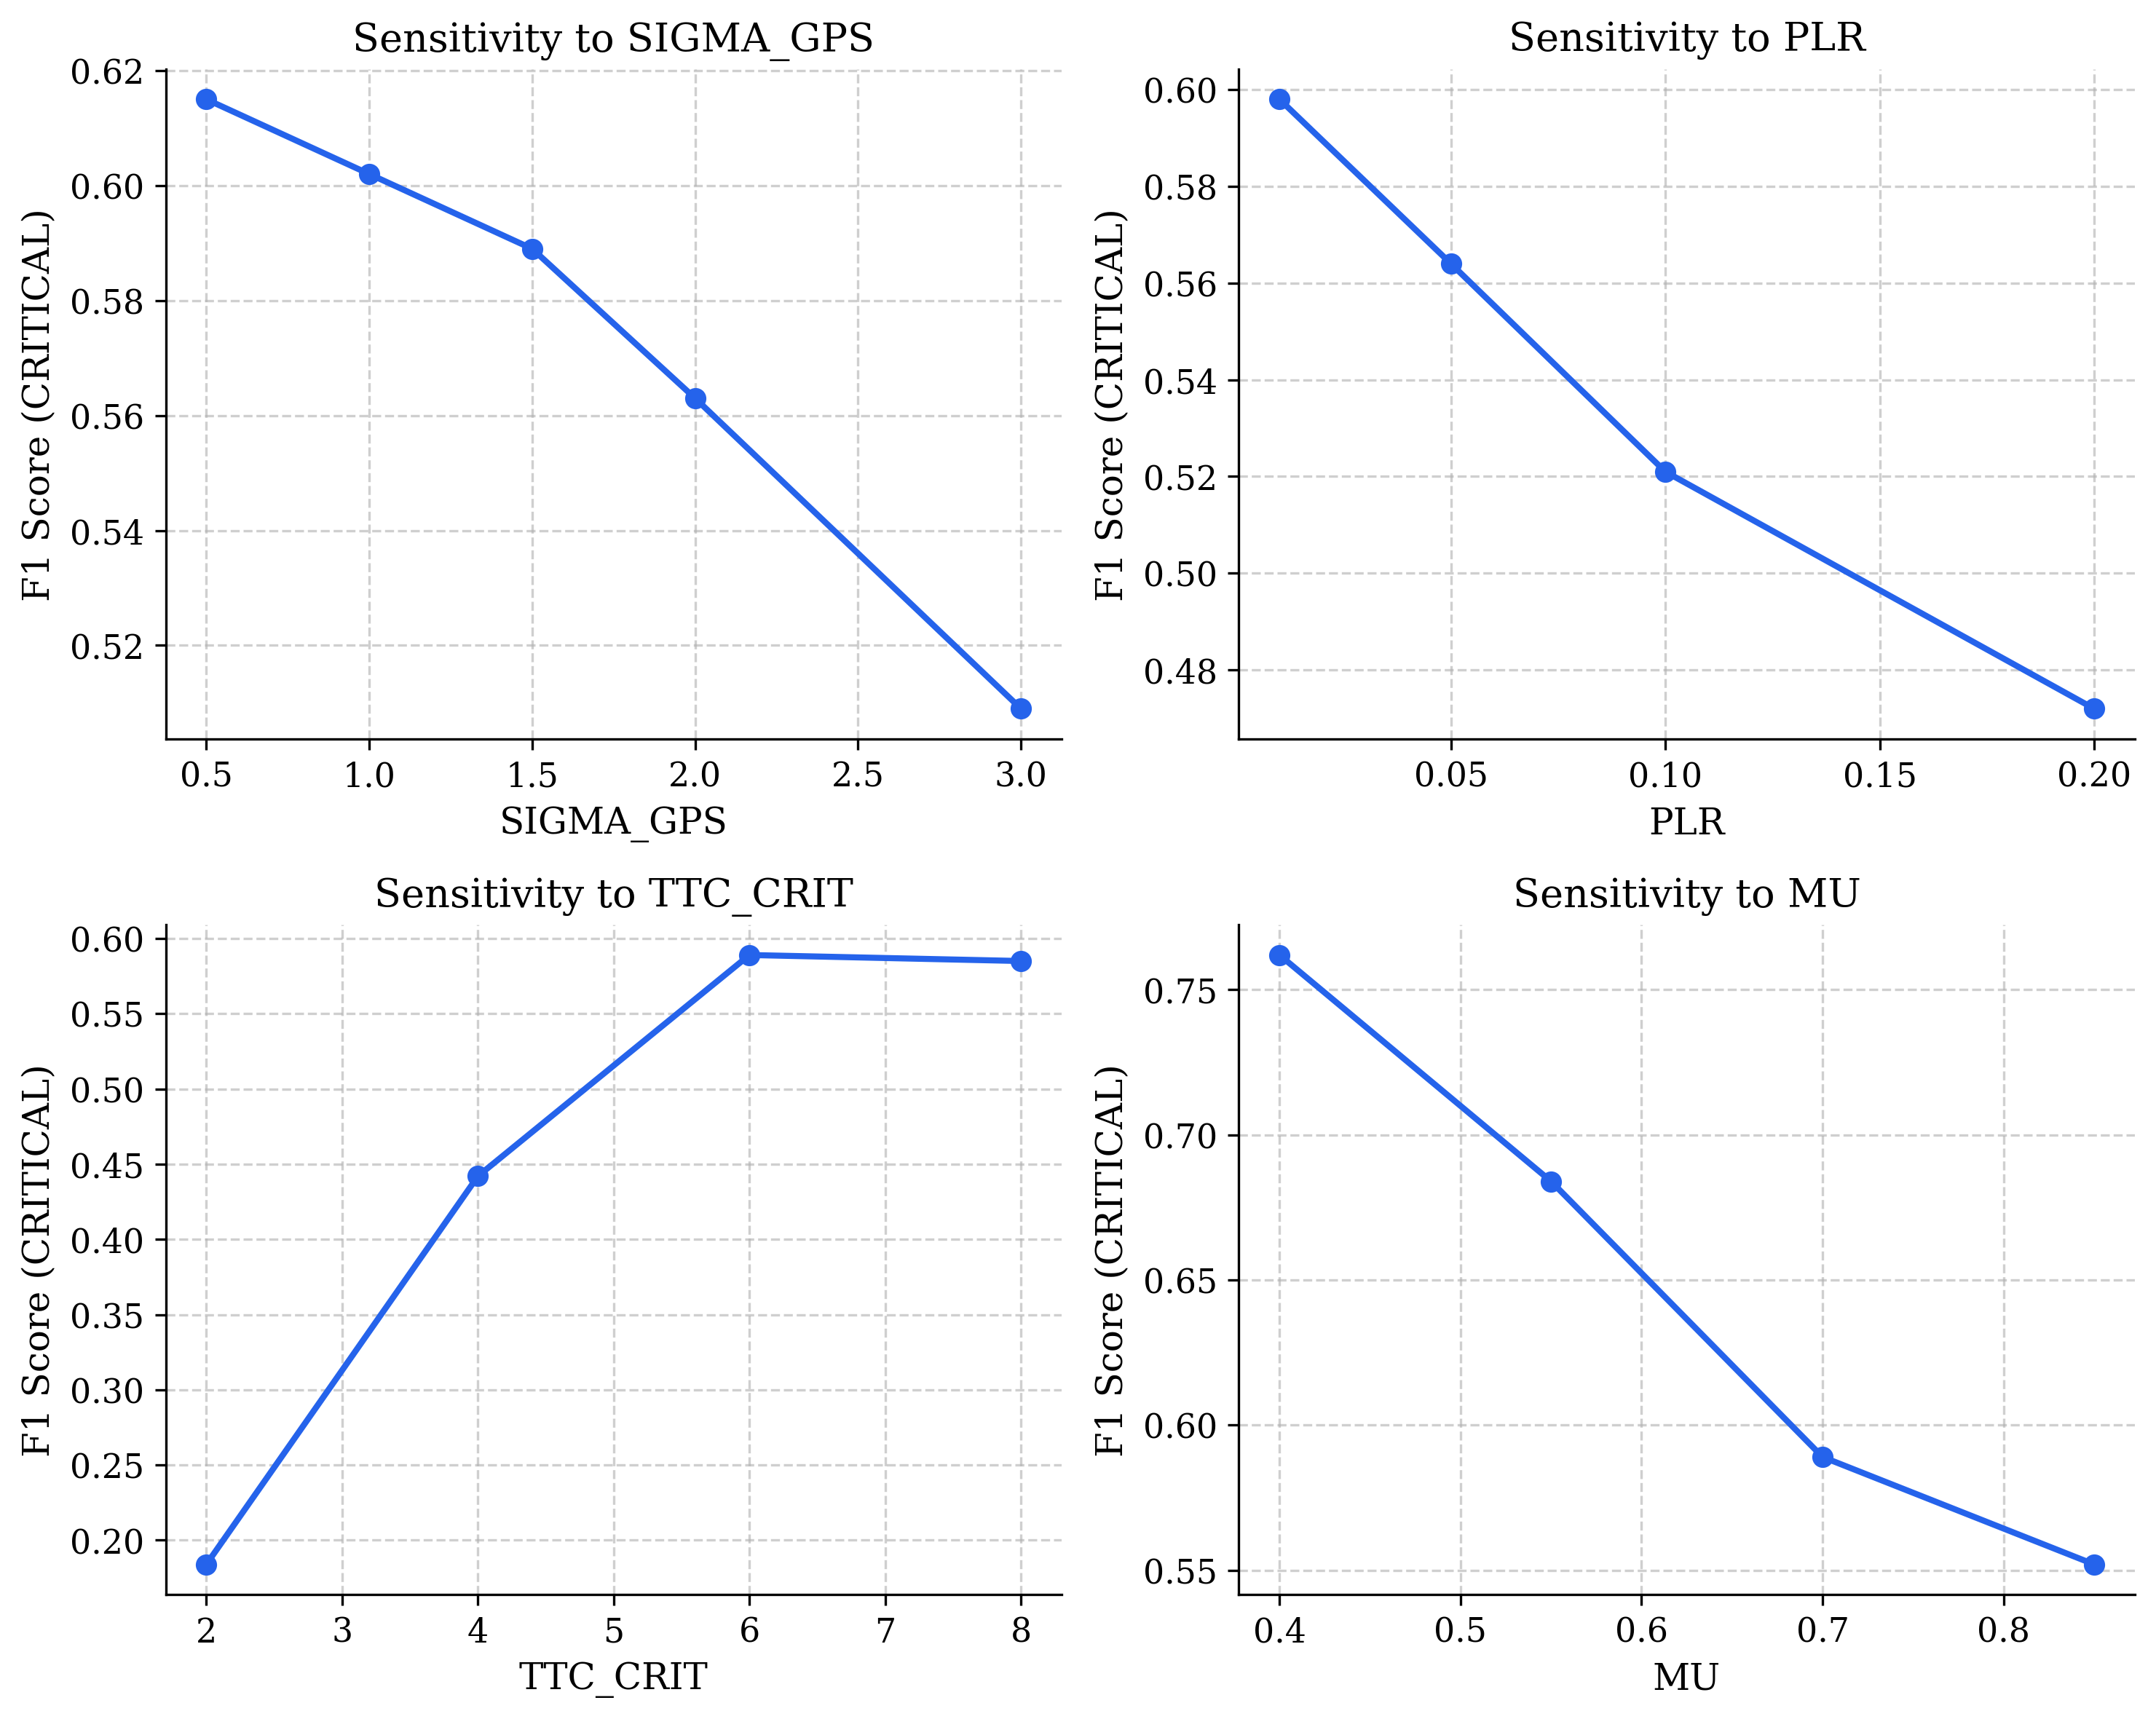
\includegraphics[width=\columnwidth]{fig8_sensitivity_analysis.png}
  \caption{Sensitivity analysis across GPS noise, packet loss, TTC threshold, alert threshold, and friction values.}
  \label{fig:sensitivity}
\end{figure}

% ============================================================
% 8. REAL-WORLD DEPLOYMENT PATHWAY
% ============================================================
\section{Real-World Deployment Pathway}\label{sec:deployment}

Deploying this system on real vehicles requires only a standard DSRC or C-V2X On-Board Unit (OBU) that can transmit the 5-field BSM. Because the system uses only position, speed, and acceleration values, it does not need access to the vehicle's internal computer network for turn signals or steering data. This makes it compatible with existing aftermarket V2V communication kits.

For embedded hardware deployment, the CRI logic has been packaged as a ROS2 node that converts GPS coordinates into the local coordinate frame used by the physics engine. A single processing cycle with 15 simultaneous targets completes in 4.7~ms, well within the 100~ms time budget required by the SAE J2945/1 standard~\cite{sae_j2945}.

The XGBoost model is exported in ONNX format for potential future embedded inference, pending improvement with additional training data. The physics model is the sole decision-maker in the current deployment configuration.

\textbf{Current status:} All results in this paper are from simulation. Hardware testing on physical vehicles is planned as future work. The ROS2 wrapper and ONNX export have been validated in software-only testing.

% ============================================================
% 9. DISCUSSION
% ============================================================
\section{Discussion}\label{sec:discussion}

The main finding is that the transparent physics model (proxy AUC = 0.9869; SUMO-collision AUC = 0.9416) significantly outperforms both traditional baselines and the exploratory XGBoost model (AUC = 0.7725) for blind-spot risk assessment, even though all methods consume the same 5-field BSM input. The severity gate --- requiring at least one physical danger signal to be genuinely high --- is the key to this result. The ablation study confirms: removing the gate by adding the unreliable intent component ($\gamma=0.20$) reduces F1 by 44\%.

The XGBoost model's underperformance relative to even the TTC kinematic baseline (0.8886) and static box baseline (0.8737) is an instructive negative result. With only 54 CRITICAL events in 146,051 observations, the classifier cannot learn the rare-event boundary that the physics model encodes via domain knowledge (stopping distance, TTC geometry). This finding supports the broader principle that for safety-critical applications with extreme class imbalance, physics-informed models with encoded domain priors outperform purely data-driven alternatives unless training data volume is substantially larger~\cite{chen2016xgboost}.

The system maintains consistent performance across normal traffic, traffic signal violations, and narrow road scenarios ($\Delta$AUC $<$ 0.002), and across six independent random traffic seeds ($\sigma=0.0041$, Table~\ref{tab:multiseed}).

\subsection{Limitations}
\begin{enumerate}
  \item \textbf{Simulation only.} Results are from traffic simulation. Real-world V2V conditions may differ.
  \item \textbf{Proxy ground truth circularity.} The kinematic near-miss proxy (Tier~2) shares structural inputs with the CRI model, which inflates the proxy-based AUC. The SUMO-collision AUC (0.9416, $n{=}27$) provides a model-independent lower bound but is based on a small sample.
  \item \textbf{No pedestrians or cyclists.} The system only detects vehicles with V2V capability.
  \item \textbf{Single road network.} Testing was done on one road network. More networks should be tested.
  \item \textbf{No turn signals.} The 5-field BSM constraint means lane-change intent cannot be reliably predicted.
  \item \textbf{Insufficient CRITICAL samples.} The simulation produced only 54 CRITICAL-class events, preventing the AI model from learning this class. Longer simulations or targeted scenario injection are needed.
  \item \textbf{No security measures.} The system trusts all received data. Fake or manipulated messages could cause incorrect risk assessments.
\end{enumerate}

% ============================================================
% 10. CONCLUSION
% ============================================================
\section{Conclusion}\label{sec:conclusion}

This paper presented a V2V Blind Spot Detection system that uses only 5 basic data fields from the standard vehicle safety message. By not requiring additional data like turn signals or yaw rate, the system works with all types of vehicles equipped with DSRC or C-V2X communication.

The core innovation is the Collision Risk Index (CRI) with a severity gate that prevents false alarms by requiring at least one physical danger signal to be genuinely high before triggering a warning. Tested over 146,051 observations on a real road network with injected danger scenarios, the physics model achieved an AUC of 0.9869 against a kinematic near-miss proxy (0.9416 against SUMO-reported collisions) --- significantly outperforming both traditional TTC (0.8886) and static box (0.8737) detection methods. An exploratory XGBoost classifier underperformed all baselines (AUC = 0.7725), demonstrating that data-driven approaches require substantially more rare-event training data to compete with physics-informed models for safety-critical detection.

Future work priorities include: (1)~testing on real vehicles with commercial V2V hardware; (2)~evaluation against real collision data to replace the proxy ground truth; (3)~longer simulations or targeted scenario injection to generate sufficient CRITICAL training samples; (4)~testing on diverse road networks; and (5)~feature set reduction to eliminate the four redundant feature pairs identified in the correlation analysis. The lightweight, transparent system provides a strong foundation for cooperative vehicle safety.

% ============================================================
% ACKNOWLEDGEMENTS
% ============================================================
\begin{acknowledgements}
The authors thank the Eclipse SUMO development team (DLR) for the open-source traffic simulation platform, and OpenStreetMap contributors for the Atal Bridge road network data.
\end{acknowledgements}

% ============================================================
% REFERENCES
% ============================================================
\begin{thebibliography}{19}

\bibitem{sae_j2735}
SAE International, ``Dedicated Short Range Communications (DSRC) Message
Set Dictionary,'' SAE Standard J2735\_202309, Sep.\ 2023.

\bibitem{sae_j2945}
SAE International, ``On-Board System Requirements for V2V Safety
Communications,'' SAE Standard J2945/1\_201603, Mar.\ 2016.

\bibitem{ieee_80211p}
IEEE, ``IEEE Standard for Information Technology --- Wireless Access in
Vehicular Environments,'' IEEE Std 802.11p-2010, Jul.\ 2010.

\bibitem{3gpp2016}
3GPP, ``Study on LTE-based V2X Services,'' 3GPP TR 36.885 V14.0.0, Jun.\ 2016.

\bibitem{euroncap2019}
Euro NCAP, ``Lane Change Assist System (LCAS) Test Protocol,'' Version 1.0, 2019.

\bibitem{aashto2018}
AASHTO, \textit{A Policy on Geometric Design of Highways and Streets},
7th ed.\ Washington, DC, 2018.

\bibitem{gilbert1960}
E.~N. Gilbert, ``Capacity of a burst-noise channel,'' \textit{Bell Syst.
Tech. J.}, vol.~39, no.~5, pp.~1253--1265, Sep.\ 1960.

\bibitem{chen2016xgboost}
T.~Chen and C.~Guestrin, ``XGBoost: A scalable tree boosting system,'' in
\textit{Proc.\ ACM SIGKDD}, San Francisco, CA, Aug.\ 2016, pp.~785--794.

\bibitem{sumo2018}
P.~A. Lopez \textit{et~al.}, ``Microscopic traffic simulation using SUMO,''
in \textit{Proc.\ IEEE ITSC}, Maui, HI, Nov.\ 2018, pp.~2575--2582.

\bibitem{who2023}
World Health Organization, ``Global Status Report on Road Safety 2023,''
WHO, Geneva, Dec.\ 2023.

\bibitem{morth2023}
MoRTH, ``Road Accidents in India 2022,'' Government of India, New Delhi,
Oct.\ 2023.

\bibitem{mousa2021}
A.~Mousa \textit{et~al.}, ``Vehicle-to-vehicle communication for blind spot
detection,'' \textit{IEEE Trans. Intell. Transp. Syst.}, vol.~22, no.~5,
pp.~3120--3131, May 2021.

\bibitem{festag2014}
A.~Festag, ``Cooperative intelligent transport systems standards in
Europe,'' \textit{IEEE Commun. Mag.}, vol.~52, no.~12, pp.~166--172, Dec.\ 2014.

\bibitem{biswas2006}
S.~Biswas, R.~Tatchikou, and F.~Dion, ``Vehicle-to-vehicle wireless
communication protocols for enhancing highway traffic safety,'' \textit{IEEE
Commun. Mag.}, vol.~44, no.~1, pp.~74--82, Jan.\ 2006.

\bibitem{smote2002}
N.~Chawla \textit{et~al.}, ``SMOTE: Synthetic minority over-sampling
technique,'' \textit{J. Artif. Intell. Res.}, vol.~16, pp.~321--357, 2002.

\bibitem{kim2015}
B.~Kim \textit{et~al.}, ``An IMM/EKF approach for enhanced multitarget
state estimation for integrated threat assessment,'' \textit{IEEE Trans.
Veh. Technol.}, vol.~64, no.~3, pp.~876--889, Mar.\ 2015.

\bibitem{rawashdeh2008}
Z.~A. Rawashdeh and S.~M.~I. Mahmud, ``A novel V2V-based blind spot
detection system,'' in \textit{Proc.\ IEEE VTC-Fall}, Calgary, AB, Sep.\ 2008,
pp.~1--5.

\end{thebibliography}

% ============================================================
% AUTHOR BIOGRAPHIES
% ============================================================
\bigskip
\noindent\textbf{Omkar Kadam} received his B.E.\ degree in Information Technology from Terna Engineering College, Navi Mumbai, India. His research interests include vehicular communication systems, intelligent transportation, and machine learning for safety-critical applications.

\bigskip
\noindent\textbf{Abhinav Prasad} received his B.E.\ degree in Information Technology from Terna Engineering College, Navi Mumbai, India. His research interests include embedded systems and V2V communication protocols.

\bigskip
\noindent\textbf{Gauri Phanse} received her B.E.\ degree in Information Technology from Terna Engineering College, Navi Mumbai, India. Her research interests include data analytics and intelligent transportation systems.

\bigskip
\noindent\textbf{Afraz Khan} received his B.E.\ degree in Information Technology from Terna Engineering College, Navi Mumbai, India. His research interests include simulation-based testing and vehicular networks.

\bigskip
\noindent\textbf{Vaishali Khairnar} is an Assistant Professor in the Department of Information Technology at Terna Engineering College, Navi Mumbai, India. Her research interests include wireless communication, vehicular ad-hoc networks (VANETs), and intelligent transportation systems.

\end{document}
